%% LyX 2.0.6 created this file.  For more info, see http://www.lyx.org/.
%% Do not edit unless you really know what you are doing.
\documentclass[11pt,twoside,english,italian]{report}
\renewcommand{\ttdefault}{mathpazo}
\usepackage[T1]{fontenc}
\usepackage[utf8]{inputenc}
\usepackage[a4paper]{geometry}
\geometry{verbose}
\setcounter{secnumdepth}{3}
\setcounter{tocdepth}{3}
\usepackage{fancybox}
\usepackage{calc}
\usepackage{amsmath}
\usepackage{amssymb}
\PassOptionsToPackage{normalem}{ulem}
\usepackage{ulem}

\makeatletter

%%%%%%%%%%%%%%%%%%%%%%%%%%%%%% LyX specific LaTeX commands.
%% Because html converters don't know tabularnewline
\providecommand{\tabularnewline}{\\}

%%%%%%%%%%%%%%%%%%%%%%%%%%%%%% User specified LaTeX commands.

\newlength\tindent
\setlength{\tindent}{\parindent}
\setlength{\parindent}{0pt}
\renewcommand{\indent}{\hspace*{\tindent}}

\providecommand{\coursename}{Logica e Algebra 2}
\providecommand{\documentsubtitle}{Appunti}
\providecommand{\annoacc}{2011-2012}
\providecommand{\principaladviser}{Prof. Alessandra Cherubini}
\providecommand{\firstauthor}{Edoardo Pasi}
\providecommand{\firstauthorid}{edogay}
\providecommand{\secondauthor}{Davide Tateo}
\providecommand{\secondauthorid}{799311}
\title{Logica e Algebra 2}
\author{\firstauthor, \secondauthor}

 
\usepackage{tikz}

\usepackage{color}   %May be necessary if you want to color links
\usepackage{hyperref}
\hypersetup{
    colorlinks=true, %set true if you want colored links
    linktoc=all,     %set to all if you want both sections and subsections linked
    linkcolor=black,  %choose some color if you want links to stand out
}

\usepackage{booktabs}
\usepackage{listings}
\lstset{columns=fullflexible}

\usepackage{wasysym}

\usepackage{amsthm}
\newtheoremstyle{note} % name
{\topsep} 	% Space above
{\topsep} 	% Space below
{\small}		% Body font
{}		% Indent amount
{\small\bfseries}% Theorem head font
{:}		% Punctuation after theorem head
{.5em}	% Space after theorem head
{}		% Theorem head spec (can be left empty, meaning ‘normal’)

\usepackage{fancyhdr}%% Cambia il carattere delle didascalie delle figure %%
\usepackage[font=small,format=plain,labelfont=bf,up,textfont=it,up]{caption}

\usepackage{comment}

%per le tabelle lunghe e particolari
\usepackage{lscape}
%include il comando per creare la pagina dei titoli
\usepackage{settings/frontesp}

\makeatother

\usepackage{babel}
\begin{document}
\titlep

\tableofcontents{}

\selectlanguage{english}%
\global\long\def\veraw#1#2#3{#1\models_{#2}#3}


\global\long\def\vera#1#2{#1\models#2}


\global\long\def\nonvera#1#2{#1\nvDash#2}


\global\long\def\nonveraw#1#2#3{#1\nvDash_{#2}#3}


\global\long\def\nonSem#1#2{#1\nvdash#2}


\global\long\def\nonTeor#1#2{\nvdash_{#1}#2}


\global\long\def\nonSemW#1#2#3{#1\nvdash_{#2}#3}


\global\long\def\verita#1#2{#1\in V(#2)}


\global\long\def\entail#1#2{#1\models#2}


\global\long\def\semantica#1#2#3{#1\vdash_{#2}#3}


\global\long\def\teolm#1#2{\vdash_{#1}#2}


\global\long\def\semGen#1#2{#1\vdash#2}


\global\long\def\boxx#1{\square#1}


\global\long\def\diam#1{\diamond#1}


\global\long\def\dia{\diamond a}


\global\long\def\boa{\boxx a}


\global\long\def\noa{\neg a}


\global\long\def\forhten#1#2#3{\forall#1#2\implies#3}


\global\long\def\implica#1#2{#1\implies#2}


\global\long\def\teorema#1{\vdash_{\Lambda}#1}


\global\long\def\teorGamma#1{\Gamma\vdash_{\Lambda}#1}


\global\long\def\teoa{\teorGamma a}


\global\long\def\teoremaDi#1{\vdash_{#1}}


\global\long\def\consist{\mbox{\ensuremath{\Lambda}}-consistente}


\global\long\def\consMax{\Lambda-consistente\: massimale}


\global\long\def\veraCanAlfa#1{\vera{M^{\Lambda}}{_{\alpha}}#1}


\global\long\def\veraCA{\vera{M^{\Lambda}}{_{\alpha}}a}


\global\long\def\veraCan#1#2{\vera{M^{\Lambda}}{_{#1}}#2}


\global\long\def\nonveraCan#1#2{\nonveraw{M^{\Lambda}}{#1}{#2}}


\global\long\def\consMaxLog#1{#1-consistente\ massimale}


\global\long\def\relazCAB#1#2{\{a\ |\ \boa\in#1\}\subseteq#2}


\global\long\def\relazCAD#1#2{\{\diamond b\ |\ b\in#2\}\subseteq#1}


\global\long\def\andoria#1{a_{1}\wedge...\wedge a#1}


\global\long\def\andbox#1{\boa_{1}\wedge\dots\wedge\boxx a#1}
\selectlanguage{italian}%




\chapter{Introduzione}

\label{cap:introduction}


\section{Intro}

Se voi signorine finirete questo corso, e se sopravviverete sarete
dispensatori di fbf e pregherete per modellizzare sistemi assurdi
in modo ancora più assurdo, ma fino a quel giorno non siete altro
che buoni annulla convinti che tutti i cretesi sono stupidi e forse
mentono.

Lasciate il formaggio fuori dall'aula.



\chapter{Formule di Logica modale e significato}

$a$ è vera nel mondo $\alpha$, e scriviamo $\mu\models_{\alpha}a$

se 
\begin{itemize}
\item $a$ è una lettera enunciativa allora deve valere $\verita a{\alpha}$ 
\item $a$ è del tipo: $a\lor b$ .... allora.... $\mu\models_{\alpha}a$
oppure $\mu\models_{\alpha}b$ 
\end{itemize}

\section{Relazione seriale}

Ip) Frame F con relazione R seriale

Ts) $\boa\implies\dia$

Dimostrazione:

Se non vale: $\veraw{\mu}{\alpha}{\boa}$ allora immediatemente si
ha la tesi in quanto l'antecedente è falso.

Se invce: $\veraw{\mu}{\alpha}{\boa}$ allora

$\forhten{\beta}{\,:\,\alpha R\beta}{\veraw{\mu}{\beta}a}$ per definizione
di box,

inoltre dato che R seriale per Ip si ha anche che $\exists\beta:\:(\alpha,\beta)\:\in R$

da cui: $\veraw{\mu}{\alpha}{\dia}$ per definizione di diamond (esiste
$\beta$ in relazione con $\alpha$ per la serialità e in $\alpha$
vale $a$ dato che $\veraw{\mu}{\alpha}{\boa}$ )\\


Ip) $\boa\implies\dia$

Ts) Frame F con relazione R seriale

\begin{center}
$ $\begin{center}  
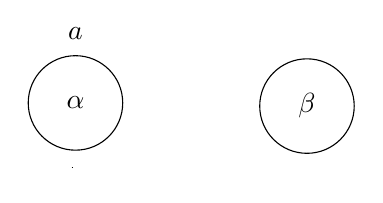
\begin{tikzpicture}[scale=0.2]  
\tikzstyle{every node}+=[inner sep=0pt]  
\draw [black] (24.2,-13) circle (3); 
\draw (24.2,-13) node {$\alpha$};
\draw (24.2,-8.6) node {$\boxx{a}$};
\draw [black] (38.9,-13.2) circle (3);
\draw (38.9,-13.2) node {$\beta$}; 
\draw (24,-17.3) node {\sout{$\dia$}};   
\end{tikzpicture} \end{center}
\par\end{center}

Per assurdo:

Suppongo di trovarmi in un mondo come quello in figura (wow) in cui
\mbox{$\veraw{\mu}{\alpha}{\boa}$ }, e suppongo che la relazione
R del frame NON sia seriale cioè $\sim\exists\beta:(\alpha R\beta)$,
se è così vale sicuramente $\veraw{\mu}a{\boa}$ (dato che $\alpha$
non ha successori) , d'altra parte per come è il mondo considerato,
cioè si nega la tesi, assurdo\sout{.}


\section{Relazione riflessiva}

Ip) R riflessiva

Ts) $\boa\implies a$

se l'antecedente è falso il teorema è dimostrato, consideriamo il
caso in cui l'antecedente è vero:

$\veraw{\mu}{\alpha}{\boa}$

poichè il frame è riflessivo, abbiamo $\alpha R\alpha$, e quindi
varrà:

$\veraw{\mu}{\alpha}a$

e la tesi è dimostrata.

\begin{center} 
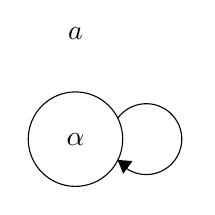
\begin{tikzpicture}[scale=0.2] 
\tikzstyle{every node}+=[inner sep=0pt] 
\draw [black] (32.4,-24.8) circle (3); 
\draw (32.4,-24.8) node {$\alpha$}; 
\draw (32.4,-20.6) node {$\boa$}; 
\draw (32.4,-18.1) node {$a$}; 
\draw [black] (35.08,-23.477) arc (144:-144:2.25); 
\fill [black] (35.08,-26.12) -- (35.43,-27) -- (36.02,-26.19); 
\end{tikzpicture} \end{center}

Ip) $\boa\implies a$

Ts) R è riflessiva

Supponiamo per assurdo che R non sia riflessiva, allora prendiamo
uno stato $\alpha$ tale che $\nexists\beta:\,\alpha R\beta$. Allora
si avrà che:

$\veraw{\mu}{\alpha}{\boa}\wedge\nonveraw{\mu}{\alpha}a$

che è assurdo perchè contraddice la tesi. La tesi allora è valida.

\begin{center} 
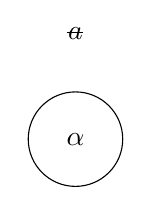
\begin{tikzpicture}[scale=0.2] 
\tikzstyle{every node}+=[inner sep=0pt] 
\draw [black] (32.4,-24.8) circle (3); 
\draw (32.4,-24.8) node {$\alpha$}; 
\draw (32.4,-20.6) node {$\boa$}; 
\draw (32.4,-18.1) node {\sout{$a$}}; 
\end{tikzpicture} 
\end{center}


\section{Relazione simmetrica}

Ip) R simmetrica

Ts) $a\implies\boxx{\dia}$

Suppongo che $\veraw{\mu}{\alpha}a$ (se no avrei già la tesi), due
casi:

\textbf{Caso 1}: Da $\alpha$ non parte nessun arco, allora sicuramente
$\veraw{\mu}{\alpha}{\boxx x}$ con $x$ qualsiasi e in particolare
$\veraw{\mu}{\alpha}{\boxx{\dia}}$

\begin{center}
\begin{center} 
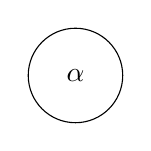
\begin{tikzpicture}[scale=0.2] 
\tikzstyle{every node}+=[inner sep=0pt] 
\draw [black] (24.2,-13) circle (3);
\draw (24.2,-13) node {$\alpha$};
\end{tikzpicture}
\end{center} 
\par\end{center}

\textbf{Caso 2}: Esiste almeno un $\beta$ tale che $\alpha R\beta$.

\begin{center}
\begin{center} 
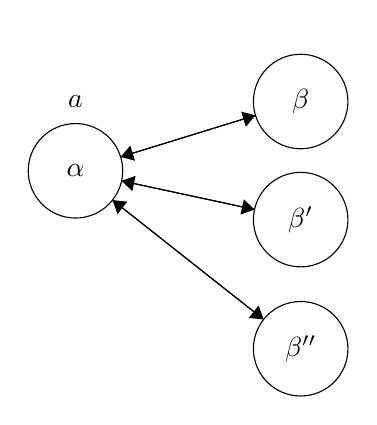
\begin{tikzpicture}[scale=0.2] 
\tikzstyle{every node}+=[inner sep=0pt] 
\draw [black] (24.2,-12.7) circle (3); 
\draw (24.2,-12.7) node {$\alpha$};
\draw (24.2,-8.3) node {$a$};  
\draw [black] (38.5,-8.3) circle (3);
 \draw (38.5,-8.3) node {$\beta$}; 
\draw [black] (38.5,-15.8) circle (3);  
\draw (38.5,-15.8) node {$\beta'$};  
\draw [black] (38.5,-24) circle (3);  
\draw (38.5,-24) node {$\beta''$}; 
\draw (38.5,-3.7) node {$\dia$};
\draw (38.5,-11.7) node {$\dia$};  \draw (38.5,-20.2) node {$\dia$}; 
\draw [black] (27.07,-11.82) -- (35.63,-9.18); \fill [black] (35.63,-9.18) -- (34.72,-8.94) -- (35.02,-9.9);  \draw [black] (35.63,-9.18) -- (27.07,-11.82);  \fill [black] (27.07,-11.82) -- (27.98,-12.06) -- (27.68,-11.1); \draw [black] (27.13,-13.34) -- (35.57,-15.16); \fill [black] (35.57,-15.16) -- (34.89,-14.51) -- (34.68,-15.48); \draw [black] (35.57,-15.16) -- (27.13,-13.34);  \fill [black] (27.13,-13.34) -- (27.81,-13.99) -- (28.02,-13.02);  \draw [black] (26.55,-14.56) -- (36.15,-22.14); \fill [black] (36.15,-22.14) -- (35.83,-21.25) -- (35.21,-22.04);  \draw [black] (36.15,-22.14) -- (26.55,-14.56);  \fill [black] (26.55,-14.56) -- (26.87,-15.45) -- (27.49,-14.66); \end{tikzpicture} \end{center}
\par\end{center}

Dato che la relazione è simmetrica se $\alpha R\beta$ allora \textbf{$\beta R\alpha$.}
Dato che $\veraw{\mu}{\alpha}a,$ in ognuno di questi $\beta$, $\beta'$,$\beta''$
ecc. vale $\dia$ perché ognuno di loro è in relazione con $\alpha$.

Allora per ognuno di questi $\beta$ si ha $\veraw{\mu}{\beta}{\dia}$,
(esiste infatti un mondo, $\alpha$, in cui vale $a$) da cui: $\veraw{\mu}{\alpha}{\boxx{\dia}}$
\\


Ip) $a\implies\boxx{\dia}$

Ts) R simmetrica

Per assurdo:

suppongo R non sia simmetrica e considero un frame con soli $\alpha$
e $\beta$ e in cui $R=\{(\alpha,\beta)\}$ . In questo frame considero
un modello con funzione di verità tale che: $V(A)=\{\alpha\}$.

In $\beta$ non vale $\dia$ perché $\beta$ non è in relazione con
nessun mondo, per questo: $\nonveraw{\mu}{\alpha}{\boxx{\dia}}$

\begin{center}
\begin{center}  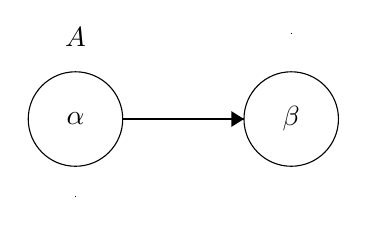
\begin{tikzpicture}[scale=0.2] \tikzstyle{every node}+=[inner sep=0pt]  \draw [black] (24.2,-12.7) circle (3);  \draw (24.2,-12.7) node {$\alpha$}; 
\draw (24.2,-7.5) node {$A$};
\draw [black] (37.9,-12.7) circle (3); \draw (37.9,-12.7) node {$\beta$};
\draw (37.9,-7.5) node {\sout{$\dia$}}; 
\draw (24.2,-17.8) node {\sout{$\boxx{\dia}$}}; 
\draw [black] (27.2,-12.7) -- (34.9,-12.7); \fill [black] (34.9,-12.7) -- (34.1,-12.2) -- (34.1,-13.2);  \end{tikzpicture} \end{center}
\par\end{center}

$ $


\section{Relazione Transitiva}

Ip) R relazione transitiva

Ts) $\boa\implies\boxx{\boa}$

Se $\nonveraw{\mu}{\alpha}{\boa}$ la tesi è dimostrata, consideriamo
allora il caso in cui $\veraw{\mu}{\alpha}{\boa}$

per ipotesi:

$\exists\beta\,:\,(\alpha,\beta)\,\in R\,(\beta,\gamma)\,\in R$

allora abbiamo che:

$(\alpha,\gamma)\,\in R$

$\veraw{\mu}{\gamma}a$ 

e quindi varrà ovviamente che:

$\veraw{\mu}{\beta}a$

da cui segue:

$\veraw{\mu}{\alpha}{\boxx{\boa}}$ 

e la tesi è dimostrata.

\begin{center} \begin{tikzpicture}[scale=0.2] 
\tikzstyle{every node}+=[inner sep=0pt] 
\draw [black] (16,-26.5) circle (3); 
\draw (16,-26.5) node {$\alpha$}; 
\draw [black] (36.8,-16.1) circle (3); 
\draw (36.8,-16.1) node {$\beta_1$}; 
\draw [black] (54.2,-25.4) circle (3); 
\draw (54.2,-25.4) node {$\gamma$}; 
\draw [black] (37.5,-38.1) circle (3); 
\draw (37.5,-38.1) node {$\beta_2$}; 
\draw (15.9,-21.5) node {$\boa$}; 
\draw (37.5,-33.4) node {$\boa$}; 
\draw (15.9,-18) node {$\boxx{\boa}$}; 
\draw (36.8,-11.9) node {$\boa$}; 
\draw (53.6,-20.6) node {$a$}; 
\draw [black] (18.68,-25.16) -- (34.12,-17.44); 
\fill [black] (34.12,-17.44) -- (33.18,-17.35) -- (33.62,-18.25); 
\draw [black] (39.45,-17.51) -- (51.55,-23.99); \fill [black] (51.55,-23.99) -- (51.08,-23.17) -- (50.61,-24.05); 
\draw [black] (19,-26.41) -- (51.2,-25.49); \fill [black] (51.2,-25.49) -- (50.39,-25.01) -- (50.42,-26.01); 
\draw [black] (18.64,-27.92) -- (34.86,-36.68); 
\fill [black] (34.86,-36.68) -- (34.39,-35.86) -- (33.92,-36.74); 
\end{tikzpicture} 
\end{center}

Ip) $\boa\implies\boxx{\boa}$

Ts) R relazione transitiva

supponiamo per assurdo che esista uno stato$\alpha$ per cui non vale
la proprietà transitiva

consideriamo il caso in cui valga la seguente funzione di valutazione:

$V(a)=\{S\,|\,(\alpha,\delta)\,\in R\}$ 

Allora a sarà vera in $\beta$, ma non in $\gamma$. per cui in $\alpha$
sarà vera $\boa$ ma non $\boxx{\boa}$

\begin{center} 
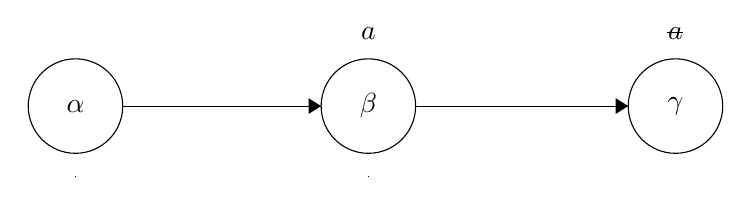
\begin{tikzpicture}[scale=0.2] \tikzstyle{every node}+=[inner sep=0pt] 
\draw [black] (16,-28.2) circle (3); 
\draw (16,-28.2) node {$\alpha$}; 
\draw [black] (34.6,-28.2) circle (3); 
\draw (34.6,-28.2) node {$\beta$}; 
\draw [black] (54.1,-28.2) circle (3); 
\draw (54.1,-28.2) node {$\gamma$}; 
\draw (16,-23.6) node {$\boa$}; 
\draw (34.6,-23.6) node {$a$}; 
\draw (54.1,-23.6) node {\sout{$a$}}; 
\draw (16,-32.9) node {\sout{$\boxx{\boa}$}}; 
\draw (34.6,-32.9) node {\sout{$\boa$}}; 
\draw [black] (19,-28.2) -- (31.6,-28.2); 
\fill [black] (31.6,-28.2) -- (30.8,-27.7) -- (30.8,-28.7); 
\draw [black] (37.6,-28.2) -- (51.1,-28.2); 
\fill [black] (51.1,-28.2) -- (50.3,-27.7) -- (50.3,-28.7); 
\end{tikzpicture} 
\end{center}




\section{Funzione parziale}

\begin{tabular}{|c|c|c|}
\hline 
$\diam a\implies\boxx a$  & funzione parziale  & $\forhten{\alpha}{:\,\alpha R\beta,\:\beta R\gamma}{\beta}=\gamma$\tabularnewline
\hline 
\end{tabular}

Funzione parziale, dimostrazione\\


Ip) funzione parziale

Ts) $\diam a\implies\boxx a$ 

$\diam{}a$ falsa allora dato che l'antecedente è falso di ha $\implica{\diam{}a}{\boxx a}$

$\diam{}a$ vera allora $\exists\beta$:$\alpha R\beta$ e$\in V(\beta)$,
ma dato che la funzione è parziale questo $\beta$ è unico !

da cui $\vera{\mu}{\implica{\diamond a}{\boxx a}}$

Ip) $\diam a\implies\boxx a$ 

Ts) funzione parziale

Per assurdo: suppongo non che la funzione non sia parziale. Se è così
$\exists\alpha:$ $\alpha R\beta,$ $\alpha R\gamma$, considero un
modello in cui V(A) = \{$\beta$ \} , $\boxx A$ non vale in $\alpha$
dato che A è falsa in $\gamma$, il che contraddice l'ipotesi (BAM!)\\
 \\
 


\section{Funzione totale}

\begin{tabular}{|c|c|c|}
\hline 
$\dia\iff\boxx a$  & funzione totale  & $\forall\alpha\exists\,!\,\beta:\:\alpha R\beta$ \tabularnewline
\hline 
\end{tabular}\\
 \\


non ci sono ``conti'' da fare, R è seriale sse R è seriale $\boxx a\implies\diam a$
, e se R è una funzione parziale $\implica{\diam a}{\boxx a}$

quindi dato che l'implica prevede un and di implica da una parte e
dall'altra per definizione abbiamo la tesi

.


\section{Relazione euclidea}

\begin{tabular}{|c|c|c|}
\hline 
$\dia\implies\boxx{\diam a}$  & relazione euclidea  & $\forhten{\alpha,\beta,\gamma}{:\:(\alpha R\beta,\:\alpha R\gamma)}{\beta}R\gamma$
da cui anche: $\beta$R$\beta$, $\gamma R\gamma$, $\gamma$R$\beta$\tabularnewline
\hline 
\end{tabular}\\
 \\


Ip) relazione euclidea

Ts) $\diam a\implies\boxx{\diam a}$

Suppongo sia vero l'antecedente (se falso ho finito), quindi vale:
$\dia$ da cui: $\vera{\mu}{\dia}$

dato che $\dia$ si ha che esiste almeno un $\beta$ tale che in beta
vale a

solo un beta: autoanello perché euclidea e quindi $\boxx{\dia}$

diversi beta: ognuno dei vari $\beta'$, $\beta''$ , ecc. sono in
relazione con $\beta$, dato che la relazione è euclidea, pertanto
dato che in $\beta$ vale $a$, in ognuno di loro vale $\dia$ \\


\begin{center}
 \begin{center}  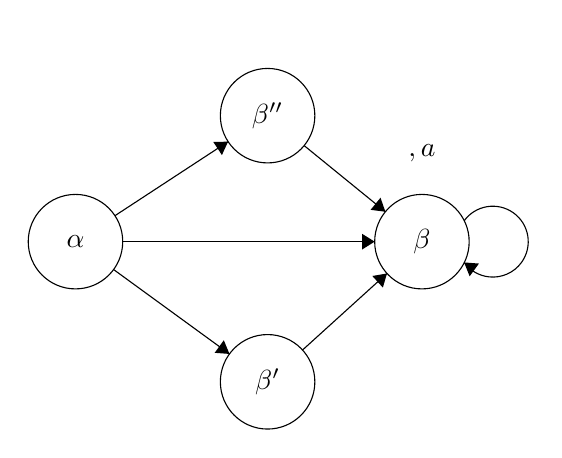
\begin{tikzpicture}[scale=0.2]  \tikzstyle{every node}+=[inner sep=0pt] \draw [black] (24.5,-18.4) circle (3); \draw (24.5,-18.4) node {$\alpha$}; \draw [black] (46.5,-18.4) circle (3);  \draw (46.5,-18.4) node {$\beta$}; \draw [black] (36.7,-27.3) circle (3);  \draw (36.7,-27.3) node {$\beta'$}; \draw (23.9,-12.8) node {$\dia$}; \draw (46.5,-12.8) node {$\dia, a$}; \draw (36.7,-22.1) node {$\dia$}; \draw [black] (36.7,-10.4) circle (3); \draw (36.7,-10.4) node {$\beta''$}; \draw (36.7,-4.9) node {$\dia$}; \draw [black] (27.5,-18.4) -- (43.5,-18.4);  \fill [black] (43.5,-18.4) -- (42.7,-17.9) -- (42.7,-18.9); \draw [black] (26.92,-20.17) -- (34.28,-25.53);  \fill [black] (34.28,-25.53) -- (33.92,-24.66) -- (33.34,-25.46);  \draw [black] (27.01,-16.75) -- (34.19,-12.05);  \fill [black] (34.19,-12.05) -- (33.25,-12.07) -- (33.8,-12.9);  \draw [black] (49.18,-17.077) arc (144:-144:2.25); \fill [black] (49.18,-19.72) -- (49.53,-20.6) -- (50.12,-19.79); \draw [black] (39.02,-12.3) -- (44.18,-16.5); \fill [black] (44.18,-16.5) -- (43.87,-15.61) -- (43.24,-16.38); \draw [black] (38.92,-25.28) -- (44.28,-20.42); \fill [black] (44.28,-20.42) -- (43.35,-20.58) -- (44.02,-21.32);  \end{tikzpicture} \end{center} 
\par\end{center}

Ip)$\dia\implies\boxx{\diam a}$

Ts) relazione euclidea

Per assurdo, suppondo valga ip) ma non la tesi

Considero un Frame in cui: $\alpha R\beta,$ $\alpha R\gamma,$ $\beta R\gamma$
ma NON $\beta R\gamma$ cioè si ha un frammento in cui non vale l'euclidea.
Poniamo che il modello sia tale che $V(A)$$=\{\gamma\}$

In queste ipotesi vale $\dia$ dato che in $\gamma$ vale $a$. In
$\beta$ non vale $a$ e neppure $\dia$ perché non ha ``uscite'',
da cui in $a$ non vale $\boxx{\dia}$ contraddicendo così l'ipotesi
(BAM!) 


\section{Relazione Debolmente Densa}

\begin{tabular}{|c|c|c|}
\hline 
$\dia\implies\diam{\diam a}$  & relazione debolmente densa  & $\forhten{\alpha,\beta}{:\:(\alpha R\beta)}{\exists\gamma:\,(\alpha R\gamma\wedge\gamma R\beta)}$\tabularnewline
\hline 
\end{tabular}

Ip) R debolmente densa

Ts) $\dia\implies\diam{\diam a}$ 

supponiamo che sia vero l'antecedente (se è falso la tesi è dimostrata)
avremo quindi:

$\veraw{\mu}{\alpha}{\dia}$

allora segue che:

$\exists\beta:\,\veraw{\mu}{\beta}a$

ma poichè la relazione è debolmente densa, si avrà che:

$\exists\gamma:\,(\alpha R\gamma\wedge\gamma R\beta)$

poichè in $\beta$ è vera a, allora segue:

$\veraw{\mu}{\gamma}{\dia}$

da cui segue:

$\veraw{\mu}{\alpha}{\diam{\dia}}$

e la tesi è dimostrata.

\begin{center} 
\begin{tikzpicture}[scale=0.2] 
\tikzstyle{every node}+=[inner sep=0pt] 
\draw [black] (18.2,-20) circle (3); 
\draw (18.2,-20) node {$\alpha$}; 
\draw [black] (47.3,-20) circle (3); 
\draw (47.3,-20) node {$\beta$}; 
\draw [black] (33.6,-32.3) circle (3); 
\draw (33.6,-32.3) node {$\gamma$}; 
\draw (18.2,-15.1) node {$\dia$}; 
\draw (18.2,-12.4) node {$\diam{\dia}$}; 
\draw (47.3,-15.1) node {$a$}; 
\draw (33.6,-36.9) node {$\dia$}; 
\draw [black] (21.2,-20) -- (44.3,-20); 
\fill [black] (44.3,-20) -- (43.5,-19.5) -- (43.5,-20.5); 
\draw [black] (20.54,-21.87) -- (31.26,-30.43); 
\fill [black] (31.26,-30.43) -- (30.94,-29.54) -- (30.32,-30.32); 
\draw [black] (35.83,-30.3) -- (45.07,-22); 
\fill [black] (45.07,-22) -- (44.14,-22.17) -- (44.81,-22.91); 
\end{tikzpicture} 
\end{center} 

Ip) $\dia\implies\diam{\diam a}$ 

Ts) R debolmente densa

Supponiamo per assurdo che R non sia debolmente densa.

Supponiamo allora che esista uno stato $\beta$ pozzo e $\alpha R\beta$
in cui sia vera a

segue che:

$\veraw{\mu}{\alpha}{\dia}$

ma avremo anche che:

$\nonveraw{\mu}{\beta}{\dia}$

e allora otteniamo:

$\nonveraw{\mu}{\alpha}{\diam{\dia}}$

che è assurdo perchè contraddice l'ipotesi, e quindi la tesi è dimostrata.

\begin{center} 
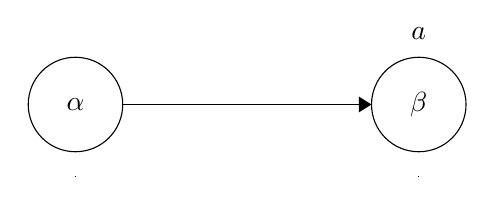
\begin{tikzpicture}[scale=0.2] 
\tikzstyle{every node}+=[inner sep=0pt] 
\draw [black] (22,-22.3) circle (3); 
\draw (22,-22.3) node {$\alpha$}; 
\draw [black] (43.8,-22.3) circle (3); 
\draw (43.8,-22.3) node {$\beta$}; 
\draw (22,-17.8) node {$\dia$}; 
\draw (43.8,-17.8) node {$a$}; 
\draw (43.8,-27.1) node {\sout{$\dia$}}; 
\draw (22,-27.1) node {\sout{$\diam{\dia}$}}; 
\draw [black] (25,-22.3) -- (40.8,-22.3); 
\fill [black] (40.8,-22.3) -- (40,-21.8) -- (40,-22.8); 
\end{tikzpicture} 
\end{center}


\section{Relazione Diretta}

\begin{tabular}{|c|c|c|}
\hline 
$\diam{\boa}\implies\boxx{\dia}$  & relazione diretta  & $\forhten{\alpha,\beta}{,\gamma:\:(\alpha R\beta\wedge\alpha R\gamma)}{\exists\delta:\,(\beta R\delta\wedge\gamma R\delta)}$\tabularnewline
\hline 
\end{tabular}

Ip) R è diretta

Ts) $\diam{\boa}\implies\boxx{\dia}$ 

Se l'antecedente è falso, il teorema è dimostrato. poniamoci quindi
nel caso:

$\veraw{\mu}{\alpha}{\diam{\boa}}$

avremo allora che:

$\exists\beta:\,\alpha R\beta\wedge\veraw{\mu}{\beta}{\boa}$

allora necessariamente si avrà che:

$\exists\delta:\,\beta R\delta\wedge\veraw{\mu}{\delta}a$

allora si avrà che:

$\veraw{\mu}{\beta}{\dia}$

prendiamo ora un qualsiasi mondo$\gamma$ tale che $\alpha R\gamma$,
poichè la relazione è diretta si avrà $\gamma R\delta$, e quindi:

$\veraw{\mu}{\gamma}{\dia}$

e allora possiamo osservare che vale:

$\veraw{\mu}{\alpha}{\boxx{\dia}}$

e la tesi è dimostrata

\begin{center} 
\begin{tikzpicture}[scale=0.2] 
\tikzstyle{every node}+=[inner sep=0pt] 
\draw [black] (17.1,-28) circle (3); 
\draw (17.1,-28) node {$\alpha$}; 
\draw [black] (33.1,-19.2) circle (3); 
\draw (33.1,-19.2) node {$\beta$}; 
\draw [black] (33.1,-38.3) circle (3); 
\draw (33.1,-38.3) node {$\gamma$}; 
\draw [black] (48,-28) circle (3); 
\draw (48,-28) node {$\delta$}; 
\draw (17.1,-23.7) node {$\diam{\boa}$}; 
\draw (33.1,-14.3) node {$\boa$}; 
\draw (48,-23.1) node {$a$}; 
\draw (33.1,-42.8) node {$\dia$}; 
\draw (17.1,-21.1) node {$\boxx{\dia}$}; 
\draw (33.1,-11.7) node {$\dia$}; 
\draw [black] (19.62,-29.62) -- (30.58,-36.68); 
\fill [black] (30.58,-36.68) -- (30.18,-35.82) -- (29.63,-36.66); 
\draw [black] (19.73,-26.55) -- (30.47,-20.65); 
\fill [black] (30.47,-20.65) -- (29.53,-20.59) -- (30.01,-21.47); 
\draw [black] (35.68,-20.73) -- (45.42,-26.47); 
\fill [black] (45.42,-26.47) -- (44.98,-25.64) -- (44.47,-26.5); 
\draw [black] (35.57,-36.59) -- (45.53,-29.71); 
\fill [black] (45.53,-29.71) -- (44.59,-29.75) -- (45.16,-30.57); 
\end{tikzpicture} 
\end{center}

Ip) $\diam{\boa}\implies\boxx{\dia}$ 

Ts) R è diretta

Supponiamo per assurdo R non diretta.

Consideriamo la funzione di valutazione:

$V(a)=\{\delta|\beta R\delta\}$

supponiamo che:

$\exists\alpha:\,\veraw{\alpha R\beta\wedge\mu}{\alpha}{\diam{\boa}}$

allora si avrà:

$\veraw{\mu}{\beta}{\boa}$

Prendiamo ora un qualsiasi mondo $\gamma$ tale che $\alpha R\gamma$,
e supponiamo che:

$\nexists\eta:\,\gamma R\eta$

Si avrà dunque che

$\nonveraw{\mu}{\gamma}{\dia}$

allora avremo che:

$\nonveraw{\mu}{\alpha}{\boxx{\dia}}$

che è assurdo, perchè contraddice la tesi. La tesi è allora valida.

\begin{center} 
\begin{tikzpicture}[scale=0.2] \tikzstyle{every node}+=[inner sep=0pt] 
\draw [black] (16.5,-26) circle (3); 
\draw (16.5,-26) node {$\alpha$}; 
\draw [black] (32.1,-15.3) circle (3); 
\draw (32.1,-15.3) node {$\beta$}; 
\draw [black] (46.9,-26) circle (3); 
\draw (46.9,-26) node {$\delta$}; 
\draw [black] (32.1,-37.6) circle (3); 
\draw (32.1,-37.6) node {$\gamma$}; 
\draw (16.5,-21.3) node {$\diam{\boa}$}; 
\draw (31.9,-10.5) node {$\boa$}; 
\draw (46.9,-21.3) node {$a$}; 
\draw (31.9,-32.8) node {\sout{$\dia$}}; 
\draw (16.5,-18.9) node {\sout{$\boxx{\dia}$}}; 
\draw [black] (18.97,-24.3) -- (29.63,-17); 
\fill [black] (29.63,-17) -- (28.68,-17.04) -- (29.25,-17.86); 
\draw [black] (34.53,-17.06) -- (44.47,-24.24); 
\fill [black] (44.47,-24.24) -- (44.11,-23.37) -- (43.53,-24.18); 
\draw [black] (18.91,-27.79) -- (29.69,-35.81); 
\fill [black] (29.69,-35.81) -- (29.35,-34.93) -- (28.75,-35.73); 
\end{tikzpicture} 
\end{center}


\section{Relazione Debolmente Connessa}

\begin{tabular}{|c|c|c|}
\hline 
$\boxx{(a\wedge\boa\implies b)}\vee\boxx{(b\wedge\boxx b\implies a)}$  & relazione debolmente connessa  & $\forhten{\alpha,\beta}{:\:(\alpha R\beta\wedge\alpha R\gamma)}{(\beta R\gamma\vee\beta=\gamma\vee\gamma R\beta)}$\tabularnewline
\hline 
\end{tabular}

Ip) R debolmente connessa

Ts) $\boxx{(a\wedge\boa\implies b)}\vee\boxx{(b\wedge\boxx b\implies a)}$

Se il primo termine è vero, il teorema è verificato. allora supponiamo
che:

$\nonveraw{\mu}{\alpha}{\boxx{(a\wedge\boa\implies b)}}$

ne consegue che:

$\nonveraw{\mu}{\beta}{a\wedge\boa\implies b}$

che si ha solo se valgono:

$\nonveraw{\mu}{\beta}b$

$\veraw{\mu}{\beta}{a\wedge\boa}$

Dobbiamo allora verificare 3 casi:

\textbf{Caso 1 }

se da $\alpha$ non esco in altri stati, poichè è falsa b, allora:

$\veraw{\mu}{\beta}{b\wedge\boxx b\implies a}$

da cui segue che:

$\veraw{\mu}{\alpha}{\boxx{(b\wedge\boxx b\implies a)}}$

E la tesi è verificata.

\begin{center} 
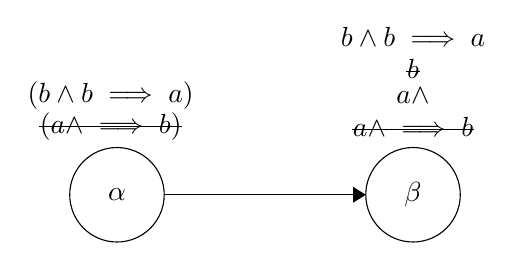
\begin{tikzpicture}[scale=0.2] 
\tikzstyle{every node}+=[inner sep=0pt] 
\draw [black] (21.9,-20.5) circle (3); 
\draw (21.9,-20.5) node {$\alpha$}; 
\draw [black] (40.7,-20.5) circle (3); 
\draw (40.7,-20.5) node {$\beta$}; 
\draw (21.5,-16.2) node {\sout{$\boxx{(a\wedge\boa\implies b)}$}}; 
\draw (21.5,-14.2) node {$\boxx{(b\wedge\boxx b\implies a)}$}; 
\draw (40.7,-16.2) node {\sout{$a\wedge\boa\implies b$}}; 
\draw (40.7,-14.2) node {$a\wedge\boa$}; 
\draw (40.7,-12.5) node {\sout{$b$}}; 
\draw (40.7,-10.5) node {$b\wedge\boxx b\implies a$}; 
\draw [black] (24.9,-20.5) -- (37.7,-20.5); 
\fill [black] (37.7,-20.5) -- (36.9,-20) -- (36.9,-21); 
\end{tikzpicture} 
\end{center}

\textbf{Caso 2 }

Se da $\alpha$ vado in un altro mondo $\gamma$ raggiungibile da
$\beta$:

$\veraw{\mu}{\gamma}a$

e quindi:

$\veraw{\mu}{\beta}{b\wedge\boxx b\implies a}$

da cui segue che:

$\veraw{\mu}{\alpha}{\boxx{(b\wedge\boxx b\implies a)}}$

E la tesi è verificata.

\begin{center} 
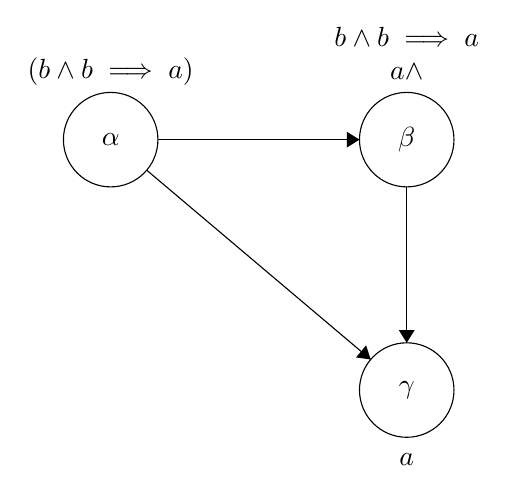
\begin{tikzpicture}[scale=0.2] 
\tikzstyle{every node}+=[inner sep=0pt] 
\draw [black] (21.9,-20.5) circle (3); 
\draw (21.9,-20.5) node {$\alpha$}; 
\draw [black] (40.7,-20.5) circle (3); 
\draw (40.7,-20.5) node {$\beta$}; 
\draw [black] (40.7,-36.4) circle (3); 
\draw (40.7,-36.4) node {$\gamma$}; 
\draw (40.7,-16.2) node {$a\wedge\boa$}; 
\draw (40.7,-40.8) node {$a$}; 
\draw (40.7,-14) node {$b\wedge\boxx{b}\implies a$}; 
\draw (21.9,-16.2) node {$\boxx{(b\wedge\boxx{b}\implies a)}$}; 
\draw [black] (24.9,-20.5) -- (37.7,-20.5); 
\fill [black] (37.7,-20.5) -- (36.9,-20) -- (36.9,-21); 
\draw [black] (40.7,-23.5) -- (40.7,-33.4); 
\fill [black] (40.7,-33.4) -- (41.2,-32.6) -- (40.2,-32.6); 
\draw [black] (24.19,-22.44) -- (38.41,-34.46); 
\fill [black] (38.41,-34.46) -- (38.12,-33.56) -- (37.48,-34.33); 
\end{tikzpicture} 
\end{center}

\textbf{Caso 3 }

Se da $\alpha$ vado in un altro mondo $\delta$ che raggiunge $\beta$:

$\nonveraw{\mu}{\delta}{\boxx b}$

e quindi, poichè è falso l'antecedente, dovrà essere:

$\veraw{\mu}{\delta}{b\wedge\boxx b\implies a}$

da cui segue che:

$\veraw{\mu}{\alpha}{\boxx{(b\wedge\boxx b\implies a)}}$

E la tesi è verificata.

\begin{center} 
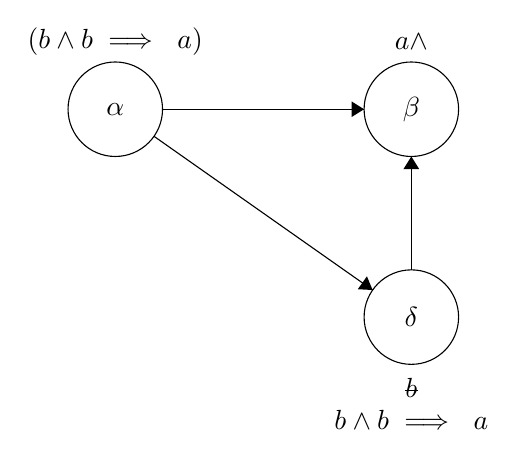
\begin{tikzpicture}[scale=0.2] 
\tikzstyle{every node}+=[inner sep=0pt] 
\draw [black] (21.9,-20.5) circle (3); 
\draw (21.9,-20.5) node {$\alpha$}; 
\draw [black] (40.7,-20.5) circle (3); 
\draw (40.7,-20.5) node {$\beta$}; 
\draw [black] (40.7,-33.7) circle (3); 
\draw (40.7,-33.7) node {$\delta$}; 
\draw (40.7,-16.2) node {$a\wedge\boa$}; 
\draw (40.7,-38.2) node {\sout{$\boxx{b}$}}; 
\draw (21.9,-16.2) node {$\boxx{(b\wedge\boxx{b}\implies\ a)}$}; 
\draw (40.7,-40.2) node {$b\wedge\boxx{b}\implies\ a$}; 
\draw [black] (24.9,-20.5) -- (37.7,-20.5); 
\fill [black] (37.7,-20.5) -- (36.9,-20) -- (36.9,-21); 
\draw [black] (24.36,-22.22) -- (38.24,-31.98); 
\fill [black] (38.24,-31.98) -- (37.88,-31.11) -- (37.3,-31.93); 
\draw [black] (40.7,-30.7) -- (40.7,-23.5); 
\fill [black] (40.7,-23.5) -- (40.2,-24.3) -- (41.2,-24.3); 
\end{tikzpicture} 
\end{center}

Ip) $\boxx{(a\wedge\boa\implies b)}\vee\boxx{(b\wedge\boxx b\implies a)}$

Ts) R debolmente connessa

Supponiamo per assurdo che R non sia debolmente connessa.

Consideriamo il caso in cui dallo stato $\alpha$ si raggiungano due
stati $\beta$ e $\gamma$, tali che $\nexists\delta:\,\beta R\delta\vee\gamma R\delta$.
Supponiamo inoltre che:

$\veraw{\mu}{\beta}{a\wedge\neg b}$

$\veraw{\mu}{\gamma}{b\wedge\neg a}$

avremo allora:

$\veraw{\mu}{\beta}{a\wedge\boa}$

$\veraw{\mu}{\gamma}{b\wedge\boxx b}$

ma, poichè l'antecedente è vero e il conseguente no, avremo anche:

$\nonveraw{\mu}{\beta}{a\wedge\boa}\implies b$

$\nonveraw{\mu}{\gamma}{b\wedge\boxx b}\implies a$

allora:

$\nonveraw{\mu}{\alpha}{\boxx{(a\wedge\boa\implies b)}\vee\boxx{(b\wedge\boxx b\implies a)}}$

che è assurdo, perchè va contro l'ipotesi. La tesi allora deve essere
valida.

\begin{center} 
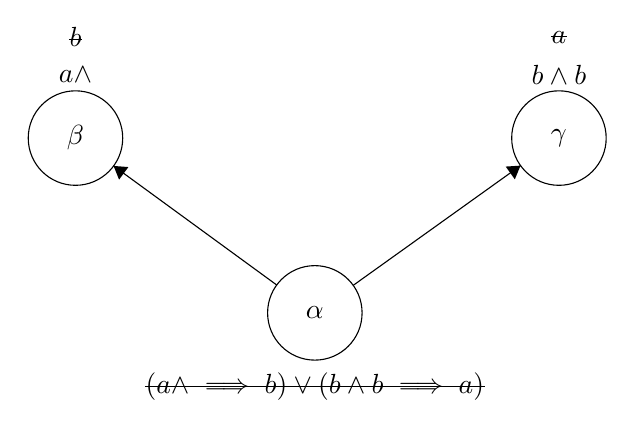
\begin{tikzpicture}[scale=0.2] 
\tikzstyle{every node}+=[inner sep=0pt] 
\draw [black] (42.2,-28.8) circle (3); 
\draw (42.2,-28.8) node {$\alpha$}; 
\draw [black] (27,-17.7) circle (3); 
\draw (27,-17.7) node {$\beta$}; 
\draw [black] (57.7,-17.7) circle (3); 
\draw (57.7,-17.7) node {$\gamma$}; 
\draw (27,-13.7) node {$a\wedge\boa$}; 
\draw (57.7,-13.7) node {$b\wedge\boxx{b}$}; 
\draw (27,-11.3) node {\sout{$b$}}; 
\draw (57.7,-11.3) node {\sout{$a$}}; 
\draw (42.2,-33.5) node {\sout{$\boxx{(a\wedge\boa\implies b)}\vee\boxx{(b\wedge\boxx b\implies a)}$}}; 
\draw [black] (44.64,-27.05) -- (55.26,-19.45); 
\fill [black] (55.26,-19.45) -- (54.32,-19.51) -- (54.9,-20.32); 
\draw [black] (39.78,-27.03) -- (29.42,-19.47); 
\fill [black] (29.42,-19.47) -- (29.77,-20.34) -- (30.36,-19.54); 
\end{tikzpicture} 
\end{center}



\chapter{Semantica}


\section{Formule equivalenti}

$a\equiv b$ cioè a è semanticamente equivalente a b, se:
\begin{itemize}
\item $\forall F\,\vera Fb\iff\vera Fa$
\item $\forall\mu\,\vera{\mu}b\iff\vera{\mu}a$
\item $\forall s\in S\,\veraw{\mu}sa\iff\veraw{\mu}sb$
\end{itemize}
si può anche dire che due formule sono semanticamente equivalenti
se:

$\vera ab\,\vee\,\vera ba$

Oppure infine se è valida in ogni frame:

$\valida{a\iff b}$


\section{Connettivi minimi}

Per ogni formula possiamo scriverne una equivalente che usa solo tre
connettivi: $\neg,\,\implies,\,\square$.

Infatti come è ben noto tutti i connettivi proposizionali si possono
esprimere in funzione della negazione e dell'implicazione, mentre
per quanto riguarda il connettivo diamond:

$\dia\equiv\neg\boxx{\neg a}$

Infatti:

se $\veraw{\mu}{\alpha}{\dia}$ allora

$\exists\beta:$$\alpha R\beta$ e $\veraw{\mu}{\beta}a$ da cui:

$\mu\nvDash_{\beta}\neg a$

per questo in $\alpha$ non vale $\boxx{\neg a}$ (perché non vale
$\neg a$ in $\beta$)

allora in $\alpha$ vale $\neg\boxx{\neg a}$ cioè $\veraw{\mu}{\alpha}{\neg\boxx{\neg a}}$
cioè la tesi. 

Similmente si dimostra l'altro verso dell'equivalenza.


\section{Logiche}


\subsection{Logica $\Lambda$}

Una logica $\Lambda$ su L è un insieme di fbf su L che: 
\begin{itemize}
\item contiene tutte le tautologie 
\item è chiusa rispetto al Modus Ponens 
\end{itemize}
Ad esempio; $PL(\phi)$ cioè i teoremi della logica proposizionale

Altro esempio $\Lambda_{C}=\{a\,|\,\vera F{a\: per}\ ogni\ F\in C\}$

infatti: 
\begin{itemize}
\item contiene tutte le tautologie perché sono vere mondo per mondo dappertutto 
\item MP : suppongo che in un mondo $\alpha$ accada che: $\nonveraw{\mu}{\alpha}b$
, $\veraw{\mu}{\alpha}a$ . Se vale anche $\veraw{\mu}{\alpha}{\implica ab}$
... l'antecedente è vero, quindi dato che l'implicazione è vera, deve
essere vero anche il conseguente da cui non può che essere $\veraw{\mu}{\alpha}b$ 
\end{itemize}
Una logica si dice \textbf{uniforme }se è chiusa rispetto a sostituzioni
uniformi cioè se sostituendo a una lettere uguali formule uguali in
una tautologia, ottengo una tautologia.

Es. $\Lambda_{C}=\{a\,|\,\vera F{a\: per}\ ogni\ F\in C\}$ NON è
uniforme infatti se considero $V(A)=S$, dove S sono tutti gli stati
possibili (mondi), vale anche $\veraw{\mu}{\alpha}A$, e cioè A è
una tautologia, se al posto di A sostituisco $B\wedge\neg B$ (falsa
in ogni modello e mondo) non ottengo una tautologia.


\subsection{Logiche modali normali}

Le logiche normali sono logiche che contengono lo schema K

$K:\,\boxx{(a\implies b)}\implies(\boa\implies\boxx b)$

Ed sono chiuse rispetto alla regola di necessitazione:

$RN:\,\dfrac{a}{\boa}$

La logica normale ha i seguenti assiomi:

$A1:\, a\implies(b\implies a)$

$A2:\,(a\implies(b\implies c))\implies((a\implies b)\implies(a\implies c))$

$A3:\,(\neg a\implies\neg b)\implies((\neg a\implies b)\implies a)$

$K:\,\boxx{(a\implies b)}\implies(\boa\implies\boxx b)$

$MP:\,\dfrac{a,\, a\implies b}{b}$

$RN:\,\dfrac{a}{\boa}$

L'intersezione di tutte le logiche normali, è una logica normale (ed
è la minima ) che non ha altri assiomi.

I teoremi sono le ultime formule della dimostrazione, ossia le formule
che ottengo dopo un numero finito di applicazione degli assiomi oppure
utilizzando la regola di necessiazione o il modus ponens.

La minima logica normale viene chiamata logica K.


\subsection{Teorema}

Sono equivalenti: 
\begin{enumerate}
\item $\Lambda$ è normale 
\item per ogni intero n $\geq0$,


$\teorema{a1\wedge a2\wedge...\wedge an}\implies a$ implica $\teorema{\boa1\wedge\boa2\wedge...\wedge\boa n}\implies\boa$

\item valgono:

\begin{enumerate}
\item $\teorema{\boxx T}$ 
\item $\teorema{\boa\wedge\boxx b}\implies\boxx{(a\wedge b)}$ 
\item $\teorema{\implica ab}$ implica $\teorema{\boa\implies\boxx b}$ 
\end{enumerate}
\end{enumerate}
Dimostrazione

$1\implies$2

per induzione.

se n = 0 allora $\teorema a$ allora $\teorema{\boa}$ per la regola
RN che vale in $\Lambda$ per ipotesi

se n > 0 (passo induttivo) suppongo valga l'antecedente, altrimenti
2 vale senz'altro;

si può dimostrare quindi nel seguente modo:

$\teolm{\Lambda}{a_{1}\wedge a_{2}\wedge...\wedge a_{n}n\implies a}$

$\teolm{\Lambda}{a_{1}\wedge a_{2}\wedge...\wedge a_{n-1}\implies(a_{n}\implies a)}$ 

$\teolm{\Lambda}{\boxx{a_{1}}\wedge\boxx{a_{2}}\wedge...\wedge\boxx{a_{n-1}}\implies\boxx{(a_{n}\implies a)}}$
-- per ipotesi di induzione

$\teolm{\Lambda}{\boxx{a_{1}}\wedge\boxx{a_{2}}\wedge...\wedge\boxx{a_{n-1}}\implies(\boxx{a_{n}\implies\boa}})$
-- per K

$\teolm{\Lambda}{\boxx{a_{1}}\wedge\boxx{a_{2}}\wedge...\wedge\boxx{a_{n-1}\wedge\boxx{a_{n}}}\implies\boa}$ 

E la tesi è dimostrata.

2$\implies$1

$\teolm{\Lambda}{(a\wedge(a\implies b))\implies b}$ -- per MP

$\teolm{\Lambda}{(\boa\wedge\boxx{(a\implies b))}}\implies\boxx b$
-- per enunciato 2

$\teolm{\Lambda}{\boxx{(a\implies b)}}\implies\boa\implies\boxx b$
-- che è K

Abbiamo ricavato usando solo il modus ponens e l'enunciato 2, l'assioma
K. segue quindi la tesi.

1$\implies3$

$\teolm{\Lambda}{\top}$

$\teolm{\Lambda}{\boxx{\top}}$-- per RN

$\teolm{\Lambda}{a\wedge b\implies a\wedge b}$ -- per tautologia
($a\implies a)$

$\teolm{\Lambda}{\boa\wedge\boxx b\implies}\boxx{(a\wedge b)}$ --
per proposizione 2

$\teolm{\Lambda}{a\implies b}$ -- per ipotesi

$\teolm{\Lambda}{\boxx{(a\implies b)}}$ -- per RN

$\teolm{\Lambda}{\boxx{(a\implies b)}\implies(\boa\implies\boxx{b)}}$
-- per K

$\teolm{\Lambda}{\boa\implies\boxx b}$ -- per MP

La tesi allora è verificata.

3$\implies$1

dimostriamo due tesi: che la 3 è chiusa rispetto alla necessitazione
e che implica l'assioma K.

$\teolm{\Lambda}a$

$\teolm{\Lambda}a\implies(\top\implies a)$ -- per A1

$\teolm{\Lambda}{\top\implies a}$ -- per MP

$\teolm{\Lambda}{\boxx{\top}\implies\boa}$ -- per 3.c

$\teolm{\Lambda}{\boa}$ -- per 3.a e MP

abbiamo così dimostrato la chiusura secondo la necessitazione.

$\teolm{\Lambda}{a\wedge b\implies c}$

$\teolm{\Lambda}{\boxx{(a\wedge b)\implies\boxx c}}$ -- per 3.c

$\teolm{\Lambda}{\boa}\wedge\boxx b\implies\boxx{(a\wedge b)}$ --
per 3.b

$\teolm{\Lambda}{\boa\wedge\boxx b\implies\boxx c}$ -- per la combinazione
delle due implicazioni precedenti

$\teolm{\Lambda}a\wedge(a\implies b)\implies b$ -- per tautologia

$\teolm{\Lambda}{\boa}\wedge\boxx{(a\implies b)}\implies\boxx b$
-- per applicazione dello schema $\boa\wedge\boxx b\implies\boxx c$
dimostrato precedentemente

$\teolm{\Lambda}{\boxx{(a\implies b)}\implies(\boa\implies\boxx{b)}}$

e così è dimostrato che K è implicato da 3. Il teorema dunque è dimostrato.


\section{Deducibilità di una formula}

Una formula a si dice deducibile da un insieme di formule $\Gamma$
in una logica $\Lambda$ e si scrive:

$\sintattica{\Gamma}{\Lambda}a$

se e solo se:

$\teorema{a_{1}\wedge\,...\,\wedge a_{n}\implies a}$

con $a_{1},\,...\,,\, a_{n}\in\Gamma$

Cioè, una formula a si dice deducibile da un insieme di formule $\Gamma$
se e solo se la congiunzione di formule che formano $\Gamma$ implica
la formula a

si noti che:

$\sintattica{\Gamma}{\Lambda}a\implies\sintattica{\{\boxx b\,|b\in\Gamma\}}{\Lambda}{\boa}$



\chapter{Verso la decidibilità - Logica determinata}


\section{Insieme $\Lambda$ consistente e sue proprietà}

Sia $\Lambda$ una logica (cioè ha tutte le tautologie ed è chiusa
rispetto al Modus Ponens)

$\Gamma$ si dice $\Lambda$-consistente se: $\nonSemW{\Gamma}{\Lambda}{\bot}$,
dove $\bot=A\wedge\neg A$

$\Delta$ si dice $\Lambda$-consistente massimale se per ogni fbf
$a$ $a\in\Delta$ oppure $\neg a\in\Delta$ $ $\\


\textbf{Proprietà:} $ $ 
\begin{enumerate}
\item Se $\teoa$ e $\Gamma\subseteq\Delta$ allora $\Delta\teorema a$.
Ovvero se alcune premesse non mi servono posso comunque metterle per
dedurre una formula 
\item Se $\teorGamma a$ e $\Lambda\subseteq\Lambda'$ allora $\Gamma\vdash_{\Lambda'}a$.
Ovvero quello che posso dedurre in una logica più scarna (es. PL)
lo posso dedurre anche in una più ricca che la contien (es. Modale) 
\item se $a\in\Gamma$ allora $\teoa$ . \\
 Infatti $\teorema{a\implies a}$ è un teorema dato che $a\implies a$
è una tautologia 
\item $\{a|\teoa\}$ è la minima logica che contiene $\Gamma\cup\Lambda$.
Infatti posso dedurre tutte le tautologie da $\Gamma$, anche se non
userò nessuna formula di $\Gamma$ ma solo quelle che già sono nella
logica $\Lambda$ $ $ 
\item Se $\teoa$ e $\{a\}$$\teorema b$ allora $\teorGamma b$ \\
 Infatti: per dedurre $a$ uso regole di inferenza, formule di $\Gamma$,
assiomi di $\Lambda$. Per arrivare in $b$ uso assiomi di $\Lambda$
e regole di inferenza, quindi posso arrivare da $\Gamma$ direttamente
in $b$ usando formule di $\Gamma$, regole di inf. e assiomi di $\Lambda$ 
\item Se $\teoa$ e $\teorGamma{\implica ab}$ allora $\teorGamma b$, dato
che $\Lambda$ è chiusa rispetto al MP 
\item $\Gamma\cup\{a\}\teorema b$ se e solo se $\teorGamma{\implica ab}$
\\
 \textbf{Andata}: $\teorema{a_{1}\wedge...\wedge a\wedge...\wedge}a_{n}\implies b$
(per definizione di teorema), si può portare $a$ alla destra dell'implicazione
$\teorema{a_{1}\wedge...\wedge}a_{n}\implies(a\implies b)$ \\
 \textbf{Ritorno}: $\teorema{a_{1}\wedge}...\wedge a_{n}\implies(a\implies b)$,
basta portare $a$ tra le $ $and. 
\item $\teoa$ se e solo se $\Gamma\cup\{\neg a\}$ non è $\Lambda$-consistente
\\
 \\
 \textbf{Andata}: $\teoa$, $\Gamma\teorema{\neg a}$, posso dedure
$\bot$ che è contro la definizione di $\Lambda$-consistenza\\
 \textbf{Ritorno}: Se$ $$\Gamma\cup\{\neg a\}$ non è $\Lambda$-consistente,
allora $\Gamma\cup\{\neg a\}\teorema{\bot}$ da cui per 7. \\
 $\Gamma\teorema{\neg a\implies\bot}$ (sposto $\neg a$ a destra
e metto l'implica), \\
 Dato che $(\neg a\implies\bot)\implies a$ è una tatutologica, per
MP ottengo\\
 $a$ 
\item $\Gamma$ è $ $$\consist$ se e solo se $\exists\beta:\nonSem{\Gamma}{_{\Lambda}\beta}$
\\
 \textbf{Andata}: Basta prendere $\neg a\wedge a$\\
 \textbf{Ritorno}: Se deducessi tutte le formule ($\neg$$\exists\beta:\nonSem{\Gamma}{_{\Lambda}\beta}$
significa $\forall\beta:\teorGamma{\beta}$) , potrei dedurre anche
$\bot$, da cui la non consistenza 
\item $\Gamma$ è $\consist$ se per ogni $a$ \\
 $\Gamma\cup\{a\}$ o $\Gamma\cup\{\neg a\}$ è $\consist$\\
 se $\teoa$ allora $ $$\Gamma\cup\{\neg a\}$ non è consistente
perché con $a$ e $\neg a$ posso dedurre $\bot$, ma $\Gamma\cup\{a\}$
lo è \\
 se $\Gamma\teorema{\neg a}$ allora $ $$\Gamma\cup\{\neg a\}$ è
consistente ma non $\Gamma\cup\{a\}$ 
\item $\bot$$\notin\Gamma$ se $\Gamma$ è $\consist$ (altrimenti potrei
dedurlo per il 3.) 
\item Se $\Delta$è $\consist\: massimale$ e $\Delta\teorema a$ allora
$a\in\Delta$\\
 se $a\notin\Delta$ allora $\neg a\in\Delta$ (dato che $\Delta$è
massimale) \\
 ma se $\Delta$ contiene $\neg a$ allora per il 2.)\\
 $\Delta\teorema{\neg a}$ , che insieme a $\Delta\teorema a$ mi
da $\Delta\teorema{\bot}$ 
\item Se $\Delta$ è $\consMax$ e $ $$a\in\Delta$. $\implica ab\in\Delta$
allora $b\in\Delta$. \\
 Lo si vede subito usando 2.) se tutti e tre, e poi 6.) (deduco $a$,
$\implica ab$, allora deduco anche $b$) 
\end{enumerate}

\section{Insieme $\Lambda$ consistente massimale}

\emph{\large{{{{Lemma di Lindelman - Esistenza dell'insieme $\consMax$}}}}}{\large{{{
}}}}\emph{\large{{{{in una logica $\Lambda$}}}}}{\large{{{
}}}}\emph{\large{{{{consistente}}}}}{\large{{{}}}}\\
 {\large{{{ }}}}\\
 {\large{{{ Considero tutte le formule $b1,\ b2,\ b3,\dots$ della
logica $\Lambda$ (posso farlo perché sono un'infinità numerabile)}}}}{\large \par}

Chiamo $\Gamma_{0}$ un insieme che contiene una sola formula (ad
esempio una tautologia)

Dopodichè iterativamente, per ogni formula mi chiedo\\


$\Gamma_{0}$$\teorema{b1}$ ? $\begin{cases}
si: & \Gamma_{1}=\Gamma_{0}\cup b1\\
no: & \Gamma_{1}=\Gamma_{0}\cup\neg b1
\end{cases}$\\


$\Gamma_{1}$$\teorema{b2}$ ? $\begin{cases}
si: & \Gamma_{2}=\Gamma_{1}\cup b2\\
no: & \Gamma_{2}=\Gamma_{1}\cup\neg b2
\end{cases}$ 
\begin{description}
\item [{$\Delta=\bigcup_{n\geq0}\Gamma_{i}$}] (nota, questa unione è infinita) 
\item [{$\Delta$}] è consistente massimale infatti:\end{description}
\begin{enumerate}
\item Massimale in quanto contiene $a$ oppure $\neg a$ per costruzione 
\item Consistente. Per assurdo se non lo fosse avrei: $\Delta\teorema{\bot}$\\
 cioè esiste un numero finito di formule di $\Delta$ da cui deduco
il falso,\\
 dato che è un numero finito di formule, sta in $\Gamma_{i}$ , cioè
esiste un $\Gamma_{i}$ non consistente, assurdo perché lo sono tutti
per costruzione \lightning 
\end{enumerate}
\emph{\large{{{Nota:}}}}{\large \par}
\begin{itemize}
\item Non sappiamo costruire $\Delta$ perché nasce da unione infinita 
\item Non è unico, infatti se considero formule in ordine diverse potrei
``dire'' si o no in modo diverso \\
 es. $a,\ \implica ab,\ b$ (allora $\Delta$ contiene $b$)\\
 es. $b,\ c$ (allora $\Delta$ contiene $\neg b$) 
\end{itemize}

\subsection{Teorema}

$\teoa$ se e solo se $a\in$ a tutti i quei $\Delta$ $\Lambda-consistenti\ massimali$
tali che: $\Gamma\subseteq\Delta$\\


\textbf{Andata:}

$\teoa$, anche $\Delta\teorema a$ per la 1.)

\textbf{Ritorno:}

Per assurdo, se $\nonSem{\Gamma}{_{\Lambda}a}$ allora $\Gamma\cup\{\neg a\}$
è $\consist$ (per la 8.)

da cui per Lindellman esiste $\Delta'$ che contiene $\Gamma\cup\{\neg a\}$
consistente massimale

data la consistenza $\Delta'$ non contiene $a$, il che è contro
l'ipotesi \lightning 


\section{Lemma di Verità}

Sia $M^{\Lambda}(S^{\Lambda},R^{\Lambda},V^{\Lambda})$ il modello
canonico di $\Lambda$

$\veraCanAlfa a$ se e solo se $a\in\alpha$\\


Ip) $\veraCanAlfa a$ 

TS) $a\in\alpha$\\


Dimostrazione per \textbf{induzione} sul numero n dei connettivi della
formula $a$

\ovalbox{n=0} cioè $a$ è del tipo $A$ (lettera enunciativa) da
cui $\veraCA$ se e solo se $\alpha\in V^{\Lambda}(A)$ se e solo
se $A\in\alpha$

\ovalbox{Ipotesi di Induzione} $a$ con n connettivi, può essere
dei seguenti tipi:
\begin{enumerate}
\item $\neg b$
\item $\implica bc$
\item $\boxx b$
\end{enumerate}
\textbf{Caso 1:} $\veraCA$ se e solo se $\veraCanAlfa{\neg b}$ se
e solo se $\nonveraCan{\alpha}b$\\


$b$ ha $n-1$ connettivi (dato che $b$) ne ha $n$, quindi vale
l'ipotesi di induzione da cui:

$b\notin\alpha$, d'altra parte $\alpha$ è $\consMax$ (per come
è definito $S^{\Lambda}$) da cui:

\textbf{$b\notin\alpha$ }se e solo se \textbf{$ $}$\neg b\in\alpha$
cioè se:

$a\in\alpha$ 

\textbf{Caso} 2:$ $ $\veraCA$ se e solo se

Caso 21: $\nonveraCan{\alpha}b$ 

Caso 22: $\veraCan{\alpha}c$\\


\textbf{Caso 21}: $\nonveraCan{\alpha}b$ \\


Il numero di connettivi di $b$ e di $c$ sommati dà $n-1$

quindi per ipotesi induttiva $\nonveraCan{\alpha}b$ se e solo se
$b\notin\alpha$ 

se e solo se $\neg b\in\alpha$ (per la compattezza max di $\Lambda$)
\textbf{({*})}

D'altra parte $\neg b\implies(b\implies c)$ è una tautologi della
PL e quindi è un teorema di $\Lambda$ (perché un logica contiene
tutte le tautologie)

e quindi $\neg b\implies(b\implies c)$ $\in\alpha$ \textbf{({*}{*})}

da cui per MP con \textbf{({*})} e \textbf{({*}{*})} si ha che $b\implies c$
appartiene ad $\alpha$\\
\\
\textbf{Caso 22}: $\veraCan{\alpha}c$\\


Vale l'ipotesi di induzione da cui:

quindi per ipotesi induttiva $\veraCan{\alpha}c$ se e solo se $c\in\alpha$
\textbf{({*})}

D'altra parte $c\implies(b\implies c)$ è una tautologi della PL e
quindi è un teorema di $\Lambda$ (perché un logica contiene tutte
le tautologie)

e quindi $c\implies(b\implies c)$ $\in\alpha$ \textbf{({*}{*})}

MP \textbf{({*}) }e \textbf{({*}{*}) }ci dà $b\implies c$ appartiene
ad $\alpha$\\
\\
\textbf{Caso 3}: $a$ è del tipo $\boxx b$

Ip)$\veraCan{\alpha}{\boxx b}$

Ts)$\boxx b\in\alpha$\\


Dall'ipotesi segue che $\forall\beta:(\alpha,\beta)\in R^{\Lambda}$
si ha: $\veraCan{\beta}b$ (questo per la definizione di $\boa$)

$b$ ha $n-1$ connettivi quindi vale per lei l'ipotesi di induzione: 

$b\in\beta$

\ovalbox{\parbox[t][1\totalheight][c]{0.9\textwidth}{%
$(\alpha,\beta)\in R^{\Lambda}$ se e solo se: $\{a\ |\ \boa\in\alpha\}\subseteq\beta$

$\alpha\in V^{\Lambda}(A)$ se e solo se: $A\in\alpha$%
}} \\


Ognuno dei $\beta$ con cui $\alpha$ è in relazione è $\consMax$
e ognuno contiene l'insieme $\{a\ |\ \boa\in\alpha\}$ 

$\Gamma\teorema a$ se e solo se $a$ appartiene a tutti i $\Delta_{i}$
$\consMax$ con $\Gamma\subseteq\Delta_{i}$

$\beta\teorema b$ se e solo se $b$ appartiene a tutti i $\Delta_{i}$
$\consMax$ con $\beta\subseteq\Delta_{i}$

$\{a\ |\ \boa\in\alpha\}$ è consistente massimale (davvero??) e quindi

$\{a\ |\ \boa\in\alpha\}$ $\teorema b$, per la 2. definizione equivalente
di Logica Normale ``aggiungo $\square$ ad entrambi i lati'' da
cui:

$\{\boa\ |\ \boa\in\alpha\}$ $\teorema b$

Ma $\{\boa\ |\ \boa\in\alpha\}$ è un sottoinsieme di formule di $\alpha$
quindi a maggior ragione ricavo $b$ da tutto $\alpha$ da cui:

$\alpha\teorema b$\\
Ip) $\boxx b\in\alpha$

TS) $\veraCanAlfa{\boxx b}$\\
Se $\boxx b\in\alpha$ per definizione di $R^{\Lambda}$ per ogni
mondo $\beta$ con $(\alpha,\beta)\in R^{\Lambda}$ si ha $b\in\beta$

Notiamo che $b$ ha $n-1$ connettivi, quindi vale l'ipotesi di induzione
e quindi:

$ $$b\in\beta$ se e solo se $\veraCan{\beta}b$

Dato che questo vale $ $per ogni $\beta$ in relazione con $\alpha$,
si ha: $\veraCanAlfa{\boxx b}$


\section{Correttezza e completezza della logica K rispetto a tutti i Frame}

Dimostriamo che la logica K (minima logica modale normale) è corretta
e completa

Ip) $\teolm Ka$ 

Ts)$\vera Fa$\\


A1, A2, A3 sono tautologie e quindi valide su tutti i frame

MP, sia la regola di necessitazione (RN) fanno passare da formule
valide su un frame a formule valide su quello stesso frame. 

Essendo $a$ l’ultima formula di una sequenza finita di fbf che o
sono istanze degli assiomi A1, A2, A3, K o sono ottenute da fbf precedenti
tramite MP o RN, è una fbf valida su ogni frame.\\
\\
Ip) $\vera Fa$

Ts)$\teolm Ka$ \\
\\
Supponiamo $\nonTeor Ka$, allora per il corollario del lemma di verità\\


\ovalbox{\parbox[t][1\totalheight][c]{0.9\textwidth}{%
Per ogni formula $a$, sia $\Lambda$ una logica, si ha $\vera{M^{\Lambda}}a$
se e solo se $\teorema a$, dove $M^{\Lambda}$ è il modello canonico%
}} \\


Si avrebbe: $\nonvera{M^{K}}a$ da cui anche

$\nonvera{F^{K}}a$, cioè $a$ non valida sul frame su cui $M^{K}$
è costruito quindi:

$\nonvera Fa$ (infatti esiste almeno un frame, $F^{K},$ in cui non
è valida $a$) il che però è contro l'ipotesi \lightning.


\section{Correttezza e completezza della logica K4 rispetto ai Frame transitivi}

Nota: K4 è costruita a partire dalla logica K a cui si aggiunge l'assioma
della transitività $\boa\implies\boxx{\boa}$ \\
Ip)$\teolm{K4}a$ 

Ts) $\entail Fa$ con F frame transitivo\\
\\
Simile al caso precedente in cui anche 4 è valido in quando il frame
è transitivo\\


Ip) $\entail Fa$ con F frame transitivo (cioè la cui relazione è
transitiva)

Ts)$\teolm{K4}a$\\
\\
Per procedere con una dimostrazione sulla falsa riga della precedente
abbiamo bisogno di dimostrare la transitività di $R^{K4}$

cioè della relazione $R^{K4}$ del modello canonico $M^{K4}=(S^{K4},R^{K4},V^{K4})$,
servirà ragionando per assurdo.\\


\textbf{Transitività di $R^{K4}$ }

se $(\alpha,\beta)\in R^{K4}$, $(\beta,\gamma)\in R^{K4}$ allora
$(\alpha,\gamma)\in R^{K4}$

cioè deve avvenire che: $\{a\ |\ \boa\in\alpha\}\subseteq\gamma$
(definizione di essere in relazione $\alpha R^{K4}\gamma$ del modello
canonico)

se $\boa\in\alpha$ , ricordando che:

$\alpha$ è un insieme $K4-consistente\ massimale$,

4 è un teorema della logica 

i teoremi di na logica appartengono a tutti gli insiemi consistenti
massimali rispetto a quella logica quindi

$\alpha$, così come ogni insieme $K4-consistente\ massimale$, contiene
anche $\boa\implies\boxx{\boa}$ (4) da cui

\selectlanguage{english}%
$\boxx{\boa}\in\alpha$\foreignlanguage{italian}{.}

$\{a\ |\ \boa\in$$\alpha\}\subseteq\beta$\foreignlanguage{italian}{
(per ipotesi $\alpha R^{K4}\beta$)}

\selectlanguage{italian}%
ma per ogni formula $\boa\in\alpha$ si ha che $\boxx{\boxx a}\in\alpha$
e quindi: $\{\boa\ |\ \boxx{\boxx a}\in\alpha\}\subseteq\beta$ da
cui $\{\boa\ |\ \boxx a\in\alpha\}\subseteq\beta$

\selectlanguage{english}%
$\{a\ |\ \boa\in$$\beta\}\subseteq\gamma$\foreignlanguage{italian}{
(per ipotesi $\beta R^{K4}\gamma$), ma le formule del tipo $\boa$
contenute in $\beta$ sono le stesse contenute in $\alpha$, quindi
si ha anche:}

$\{a\ |\ \boa\in$$\alpha\}\subseteq\gamma$\foreignlanguage{italian}{
cioè $(\alpha,\gamma)\in R^{K4}$ }\\
\foreignlanguage{italian}{}\\
\foreignlanguage{italian}{A questo punto possiamo usare in modo profiquo
il corollario del lemma di verità.}

\selectlanguage{italian}%
Dimostriamo la tesi per assurdo: supponiamo che $\nonTeor{K4}a$

allora per il corollario del teorema di verità si avrebbe anche $\nonvera{M{}^{K4}}a$ 

e in particolare si avrebbe $\nonvera{F^{K4}}a$, cioè si avrebbe
un Frame transtivo (infatti $R^{K4}$ è transitiva) nel quale non
è valida $a$

ma ciò contraddice l'ipotesi $\entail Fa$ (con $F$ transitivo) \lightning\\



\section{Teorema di Raggiungibilità}

$(\alpha,\beta)\in R^{\Lambda}$ se e solo se $\relazCAB{\alpha}{\beta}$
se e solo se \foreignlanguage{english}{$\relazCAD{\alpha}{\beta}$}
\\
Ip)$\relazCAB{\alpha}{\beta}$

Ts)$\relazCAD{\alpha}{\beta}$\\


Per assurdo supponiamo che

$b\in\beta$ e che $\diamond b\notin\alpha$, 

\selectlanguage{english}%
$\neg\diamond b\in\alpha$\foreignlanguage{italian}{ (dato che $\alpha$)
è $\consMax$}

\selectlanguage{italian}%
$\boxx{\neg b\in\alpha}$ (equivalenza $\boxx{\neg a}$ $\equiv$$\neg\dia$)
da cui

$\neg b\in\beta$ (definizione di $\boxx x$ e considerato $\alpha R^{\Lambda}\beta$)

il che è assurdo perché $b\in\beta$, e $\beta$ è $\consMax$\lightning\\


Ip)$\relazCAD{\alpha}{\beta}$

Ts)$\relazCAB{\alpha}{\beta}$\\
Per assurdo supponiamo cioè che

$\boa\in\alpha$ e $a\notin\beta$

$\neg a\in\beta$ (dato che $\beta$ è $\consMax$)

$\diamond\neg a\in\alpha$ (infatti $\alpha R^{\Lambda}\beta$ e in
$\beta$ è vera $\neg a$, quindi $a$ ha almeno un successore nel
quale $\neg a$ è vera)

$\neg\boxx{a\in\alpha}$ contro l'ipotesi della consistenza e massimalità
di $\alpha$\lightning\\





\begin{savequote}[60mm]
Se io avessi un mondo come piace a me, là tutto sarebbe assurdo: niente sarebbe com'è, perché tutto sarebbe come non è, e viceversa! Ciò che è, non sarebbe e ciò che non è, sarebbe! 
\qauthor{Lewis Carroll} \end{savequote}


\chapter{Logiche modali particolari e Determinatezza}

Per il teorema di correttezza e completezza abbiamo che $\teorema a$
se e solo se $\vera{M^{\Lambda}}a$

Il problema di $\vera{M^{\Lambda}}a$ è che non so costruire a livello
``pratico'' il modello canonico dato che i suoi mondi sono infiniti.

Provo quindi a vedere se $\teorema a$ se e solo se $\vera{F^{\Lambda}}a$
possa valere almeno per particolari classi di frame.\\


\shadowbox{\parbox[c]{1\textwidth}{%
\textbf{Nota: }Per dimostrare la determinatezza di una logica rispetto
a una classe di frame con una proprietà si può mostrare che la relazione
del Frame canonico costruito da quella logica gode della stessa proprietà.

Con questa chiave di lettura diamo alcune dimostrazioni di determinatezza.%
}}


\section{Serialità del frame canonico di KD}

$R^{KD}$ è seriale se: $\forall\alpha\in S^{KD}\exists\beta:(\alpha,\beta)\in R^{KD}$

TS) $\teoremaDi{KD}a$ se e solo se $R^{KD}$ è seriale

$\relazCAB{\alpha}{\beta}$ se e solo se $\alpha$ e $\beta$ sono
in relazione.

Vogliamo quindi provare che per ogni insieme $\{a\ |\ \boa\in\alpha\}$
esiste un $\beta$ che sia $KD-consistente\ massimale$ che lo contiene,

per farlo mi basta mostrare che esiste un insieme $\beta_{0}$ consistente
che lo contiene, poi per il teorema di Lindelmann saprò anche che
ne esiste uno consistente massimale.\\


$\beta_{0}=\{a\ |\ \boa\in\alpha\}$ , dimostro che $\beta_{0}$ è
consistente.

Se per assurdo non lo fosse

$\teoremaDi{KD}\andoria{_{n}\implies\bot}$, dove $a_{1},a_{2},...,a_{n}$
sono formule di $\beta_{0}$

(da cui spostando $a_{n}$ dopo l'implica)

$\teoremaDi{KD}\andoria{_{n-1}\implies\neg a_{n}}$ (uso la definizione
2. di logica normale)

$\teoremaDi{KD}\andbox{_{n}}\implies\boxx{\neg a_{n}}$

$\andbox{_{n}}\implies\boxx{\neg a_{n}}\in\alpha$ (dato che $\alpha$
è $\consMaxLog{KD}$ contiene tutti i teoremi di $KD$)

$\andbox{_{n}}\in\alpha$ per costruzione di $\beta_{0}$ (in $\beta_{0}$
valgono tutto le $\boxx x$ se $x$ vale in $\alpha)$

$\boxx{\neg a_{n}}\in\alpha$ (per MP dalle due precedenti)

$\neg\dia_{n}\in\alpha$

$\boa_{n}\in\alpha$ \textbf{({*})}

$\boa_{n}\implies\dia_{n}$ (schema seriale) \textbf{({*}{*})}

Per MP fra \textbf{({*}) }e\textbf{ ({*}{*}) }si ha $\dia_{n}\in\alpha$

\noindent \begin{flushleft}
Da cui $\alpha$ non consistente, assurdo. \lightning
\par\end{flushleft}


\section{\noindent Debole densità del frame canonico di K$X\diamond$}

\noindent \begin{flushleft}
$R$ è debolmente densa se: $\forhten{\alpha,\beta}{:\:(\alpha R\beta)}{\exists\gamma:\,(\alpha R\gamma\wedge\gamma R\beta)}$
\par\end{flushleft}

Chiamiamo K$X\diamond$ una logica costruita a partire dalla logica
$K$ aggiungendo lo schema $X\diamond$: $\dia\implies\diam{\diam a}$

La partenza del ragionamento è simile a quello del precedente in cui
come insieme considero:

$\gamma_{0}=\{a\ |\ a\in\alpha\}\cup\{\diamond b\ |\ b\in\beta\}$\\


Per assurdo:

$\teoremaDi{KX\diamond}\andoria{_{n}\wedge\diam{b_{1}\wedge...\wedge\diam{b_{n}}}}\implies\bot$

dove $a_{1},...,a_{n}$ sono formule di $\alpha$, e $b_{1},...,b_{n}$
sono formule di $\beta$

$\teoremaDi{KX\diamond}\andoria{_{n}}\implies\neg(\diamond b_{1}\wedge...\wedge\diamond b_{n})$

pongo $b=b_{1}\wedge...\wedge b_{n}$\\


\textbf{Teorema al volo:}

$\teoremaDi{KX\diamond}\neg(\diamond c\wedge\diamond d)\implies\neg\diamond(c\wedge d)$,
cioè:

\textbf{$\teoremaDi{KX\diamond}\diamond(c\wedge d)\implies\diamond c\wedge\diamond d$}\\
 infatti, sono tautologie della logica proposizionale: $\neg c\implies\neg c\vee\neg d$

e $\neg d\implies\neg c\vee\neg d$,

queste sono anche teoremi di $\Lambda$

dato che $\Lambda$ è normale si ha \foreignlanguage{english}{$\boxx{\neg c}\implies\boxx{\neg c\vee\neg d}$}
(definizione 3.3 di logica normale)

e lo stesso vale per la seconda $\boxx{\neg d}\implies\boxx{\neg c\vee\neg d}$

dato che il conseguente si ha per due antecedenti diversi allora:

\selectlanguage{english}%
$\boxx{\neg c}\vee\boxx{\neg d\implies}\boxx{\neg c\vee\neg d}$\foreignlanguage{italian}{
da cui negando e scambiando antecedente e conseguente:}

\selectlanguage{italian}%
$\neg(\boxx{\neg c\vee\neg d})\implies\neg(\boxx{\neg c}\vee\boxx{\neg d)}$,
sviluppo il $\neg$

$\diamond(c\wedge d)\implies\diamond c\wedge\diamond d$\\


Uso il teorema ottenendo (in un certo senso ``portiamo fuori'' il
$\diamond$)

\selectlanguage{english}%
$\teoremaDi{KX\diamond}\andoria{_{n}}\implies\neg\diamond(b_{1}\wedge...\wedge\diamond b_{n})$\foreignlanguage{italian}{
cioè (per come ho posto b)}

\selectlanguage{italian}%
$\teoremaDi{KX\diamond}\andoria{_{n}}\implies\neg\diamond b$

Uso la definizione 2. di logica normale e riscrivo:

$\teoremaDi{KX\diamond}\andbox{_{n}}\implies\boxx{\neg\diamond b}$

$\teoremaDi{KX\diamond}\andbox{_{n}}\implies\neg\diamond\diamond b$

dato che $\andbox{_{n}}\implies\neg\diamond\diamond b\in\alpha$

e che: $\andbox{_{n}\in\alpha}$

anche $\neg\diamond\diamond b\in\alpha$ (MP dalle due precedenti)

dato che $\diamond b\in\alpha$ anche $\diamond\diamond b\in\alpha$
per lo schema delle relazioni debolmente dense

il che ci porterebbe alla non massimalità di $\alpha$ contro l'ipotesi.
\lightning


\section{Riflessività del frame canonico di KT}

$R^{KT}$ è riflessiva se: $\forall\alpha,\,\alpha R^{KT}\alpha$

Vogliamo dimostrare che l'insieme $\{a\,|\,\boa\in\alpha\}$ di formule
è contenuto in $\alpha$

Se $\boxx a\in\alpha$ cioè se $\teoremaDi{KT}\boxx a$ allora

$\teoremaDi{KT}x$ dato che $\boxx{a\implies a}$ è uno schema della
logica $KT$ e quindi:

$a\in\alpha$.

Per questi motivi $\{a\,|\,\boa\in\alpha\}$ è in effetti contenuto
in $\alpha$

Da cui segue la tesi.


\section{Simmetria del frame canonico di KB}

$R^{KB}$è simmetrica se $\forhten{\alpha,\beta}{\,\alpha R^{KB}\beta}{\beta R^{KB}\alpha}$

Se $\beta R^{K4}\alpha$ allora:

$\{\diam b\,|\, b\in\alpha\}\subseteq\beta$

per definizione di R del modello canonico.

Dal momento che vale l'assioma B: $a\implies\boxx{\dia}$,

per ogni formula $b\in\alpha$ si ha che:

$\boxx{\diam b\in\alpha}$,

D'altra parte ogni volta che $b\in\alpha$, $\diamond b\in\beta$
dato che $\beta R^{K4}\alpha$ e quindi:

$\relazCAB{\alpha}{\beta}$ cioè $\alpha R\beta$


\section{Correttezza e completezza di KD}

La logica KD è corretta e completa rispetto alla classe dei Frame
seriali

Dimostrazione

Ip) $\vera Fa$ con F seriale

Ts) $\teoremaDi{KD}a$\\


Se a è un teorema di KD, è ricavato da una serie di formule che possono
essere applicazioni degli schemi A1, A2, A3, K, D oppure applicazioni
del modus ponens o della regola di necessitazione.

Supponiamo per assurdo che:

$\nonTeor{KD}a$

allora avremo che:

$\nonvera{\mu^{KD}}a$

e quindi:

$\nonvera{F^{KD}}a$

Poiché a non è vera nel frame canonico, non può essere vera in alcun
frame seriale, ma questo va contro l'ipotesi, assurdo. Allora la tesi
deve essere valida.



\chapter{Decidibilità Delle Logiche Modali}


\section{Filtrazione}

Dato una logica $\Lambda$ e una formula a, si può garantire che esiste
un modello $\mu$, con un numero di mondi limitato da f(n), con n
numero di sottoformule di a tale che:

$\teoremaDi{\Lambda}a\iff\vera{\mu}a$

Dimostrazione.

Ip) $a\in\Gamma\implies sottoformule(a)\subseteq\Gamma$

Ts) $\exists\mu:\,\teoremaDi{\Lambda}a\iff\vera{\mu}a$

sia $\mu$=(S,R,V), consideriamo la seguente relazione:

$\sim_{\Gamma}\subseteq S\times S$

che gode della seguente proprietà:

$\Gamma_{\alpha}=\{a\in\Gamma\,|\,\veraw{\mu}{\alpha}a\}$

$\alpha\sim_{\Gamma}\beta\iff\Gamma_{\alpha}=\Gamma_{\beta}$

Si può notare che $\sim_{\Gamma}$ è una relazuione di equivalenza,
Infatti:
\begin{enumerate}
\item è simmetrica\\
$\alpha\sim_{\Gamma}\alpha\iff\Gamma_{\alpha}=\Gamma_{\alpha}$
\item è riflessiva\\
$\alpha\sim_{\Gamma}\beta\iff\Gamma_{\alpha}=\Gamma_{\beta}\iff\beta\sim_{\Gamma}\alpha$
\item è transitiva:\\
$\alpha\sim_{\Gamma}\beta\wedge\alpha\sim_{\Gamma}\gamma\iff\Gamma_{\alpha}=\Gamma_{\beta}=\Gamma_{\gamma}\iff\gamma\sim_{\Gamma}\beta$
\end{enumerate}
Posso allora considerare l'insieme quoziente:

$S_{\Gamma}=S/\sim_{\Gamma}$

Si può dimostrare con il teorema di fattorizzazzione delle applicazioni
che:

$|S_{\Gamma}|\leq2^{|\Gamma|}$

\begin{center} 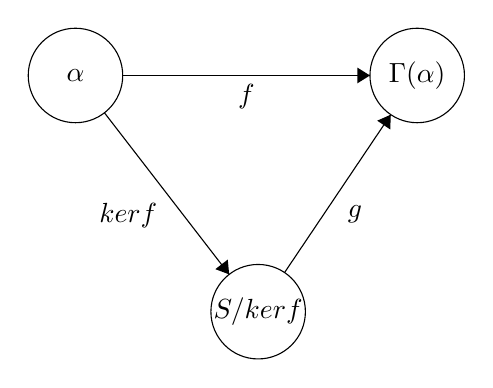
\begin{tikzpicture}[scale=0.2] \tikzstyle{every node}+=[inner sep=0pt] \draw [black] (22.1,-16.4) circle (3); \draw (22.1,-16.4) node {$\alpha$}; \draw [black] (43.8,-16.4) circle (3); \draw (43.8,-16.4) node {$\Gamma(\alpha)$}; \draw [black] (33.7,-31.4) circle (3); \draw (33.7,-31.4) node {$S/kerf$}; \draw [black] (35.38,-28.91) -- (42.12,-18.89); \fill [black] (42.12,-18.89) -- (41.26,-19.27) -- (42.09,-19.83); \draw (39.36,-25.24) node [right] {$g$}; \draw [black] (25.1,-16.4) -- (40.8,-16.4); \fill [black] (40.8,-16.4) -- (40,-15.9) -- (40,-16.9); \draw (32.95,-16.9) node [below] {$f$}; \draw [black] (23.94,-18.77) -- (31.86,-29.03); \fill [black] (31.86,-29.03) -- (31.77,-28.09) -- (30.98,-28.7); \draw (27.33,-25.31) node [left] {$kerf$}; \end{tikzpicture} \end{center}

Per dimostrarlo basta prendere:

$f:\,\alpha\rightarrow\mathcal{P}(\Gamma)$

risulta banale verificare che:

$ker\, f\equiv\sim_{\Gamma}$

e quindi, ricordando che g è iniettiva, risulta banale che:

$|S/\sim_{\Gamma}|\leq\Gamma(\alpha)$

Allora possiamo prendere il modello:

$M^{\Gamma}=(S^{\Gamma},R',V^{\Gamma})$

$R'\subseteq S^{\Gamma}\times S^{\Gamma}$

con R' che soddisfi le seguenti proprietà:

F1) $(\alpha,\,\beta)\in R\implies([\alpha],\,[\beta])\in R'$

F2) $([\alpha],[\beta])\in R'\implies\forall\boxx b\in\Gamma,\,\veraw{\mu}{\alpha}{\boxx b}\implies\veraw{\mu}{\beta}b$

Una relazione che gode delle proprietà F1 e F2 si chiama $\Gamma$-filtrazione
della relazione R.

prendiamo infine:

$V^{\Gamma}:\,\Phi\cap\Gamma\rightarrow\mathcal{P}(S^{\Gamma})$

che gode della seguente proprietà:

presa una formula atomica $A\in\Phi\cap\Gamma$

$\alpha\in V^{\Gamma}(A)\iff\alpha\in V(A)$


\subsection{Teorema}

Esiste almeno una relazione che gode delle proprietà F1 e F2:

$R^{\sigma}\subseteq S^{\Gamma}\times S^{\Gamma}$

così definita:

$([\alpha],[\beta])\in R^{\sigma}\iff\exists\delta\in[\alpha],\eta\in[\beta]\,:\,(\delta,\,\eta)\in R$

La proprietà F1 è dimostrata banalmente.

Dimostriamo F2

Ip) $([\alpha],[\beta])\in R^{\sigma}$, $\boxx{b\in\Gamma}$, $\veraw{\mu}{\alpha}{\boxx b}$

Ts) $R^{\delta}$gode della proprietà F2

supponiamo che:

$\exists\delta,\eta\,:\,\delta R\eta\wedge\delta\in[\alpha]\wedge\eta\in[\beta]$

avremo che:

$\veraw{\mu}{\delta}{\boxx b}$

$\veraw{\mu}{\eta}b$

e quindi:

$\veraw{\mu}{\beta}b$\\



\section{Lemma di Filtrazione}

dato un insieme$\Gamma$ chiuso rispetto alle sottoformule di a, con
$a\in\Gamma$

$\veraw{\mu}{\alpha}{a\iff}\veraw{\mu^{\Gamma}}{\alpha}a$

per ogni $\mu^{\Gamma}$$\Gamma$-filtrazione di $\mu$

Dimostrazione:

Ts) $\veraw{\mu}{\alpha}{a\iff}\veraw{\mu^{\Gamma}}{[\alpha]}a$

Ip) $\mu^{\Gamma}$$\Gamma$-filtrazione di $\mu$

Per induzione sul numero di connettivi di a

Caso Base, n=0:

a non ha connettivi, allora $a\equiv A$

$\veraw{\mu}{\alpha}A\iff\alpha\in V(A)\iff\alpha\in V^{\Gamma}(A)\iff\veraw{\mu^{\Gamma}}{[\alpha]}a$

Ipotesi di induzione: il teorema vale per ogni formula di $\Gamma$
con m<n connettivi.

a può essere:
\begin{enumerate}
\item $\neg b$
\item $b\implies c$
\item $\boxx b$
\end{enumerate}
Caso 1:

$\veraw{\mu}{\alpha}{\neg b}\iff\nonveraw{\mu}{\alpha}b\iff\nonveraw{\mu^{\Gamma}}{[\alpha]}b\iff\veraw{\mu^{\Gamma}}{[\alpha]}{\neg b}$

Caso 2:

$\veraw{\mu}{\alpha}{b\implies c}$ se e solo se $\nonveraw{\mu}{\alpha}b$
oppure $\veraw{\mu}{\alpha}c$

quindi si può affermare

$\nonveraw{\mu}{\alpha}b\iff\nonveraw{\mu^{\Gamma}}{[\alpha]}b$

$\veraw{\mu}{\alpha}c\iff\veraw{\mu^{\Gamma}}{[\alpha]}c$

ma vale almeno una delle due se e solo se

$\veraw{\mu^{\Gamma}}{[\alpha]}{b\implies c}$

Caso 3:

Ip) $\veraw{\mu}{\alpha}{\boxx b}$

Ts) $\veraw{\mu^{\Gamma}}{[\alpha]}{\boxx b}$

Consideriamo la reazione R' avente le proprietà F1 e F2

$\forall[\beta]\,:\,([\alpha],\,[\beta])\in R'\implies\veraw{\mu^{\Gamma}}{[\beta]}b$
-- per F2

allora si può affermare che:

$\veraw{\mu}{\beta}b\implies\veraw{\mu^{\Gamma}}{[\beta]}b\implies\veraw{\mu^{\Gamma}}{[\alpha]}{\boxx b}$

Ip)$\veraw{\mu^{\Gamma}}{[\alpha]}{\boxx b}$

Ts)$\veraw{\mu}{\alpha}{\boxx b}$

$\forall[\beta]\,:\,(\alpha,\,\beta)\in R,\,([\alpha],\,[\beta])\in R'$
--per F1

allora si può affermare che:

$\veraw{\veraw{\mu^{\Gamma}}{[\beta]}b\implies\mu}{\beta}b\implies\veraw{\mu}{\alpha}{\boxx b}$


\section{Determinatezza di K dai Frame Finiti}

La minima logica normale K è determinata dalla classe di tutti i frame
finiti.

Se $a$ ha n sottoformule $a$ è un teorema di K se e solo se A è
valida in tutti i frame con meno di $2^{n}$ mondi. 

$\teoremaDi Ka$ se e solo se $\vera Fa$.\\


Ip)$\teoremaDi Ka$ 

Ts)$\vera Fa$\\


Se $a$ è un teorema di K allora $a$ è valida in tutti i frame (infatti
K è determinata rispetto alla classe di tutti i frame) è a maggior
ragione valida in tutti i frame finiti ed in tutti i frame con meno
di $2^{n}$ mondi.\\


Ip)$\vera Fa$

Ts)$\teoremaDi Ka$\\
\\
Suppongo per assurdo che$\nonTeor Ka$ se e solo se $\nonvera{M^{K}}a$
se e solo se (per il lemma di filtrazione) $\nonvera{(M^{K})^{\Gamma}}a$
il che implica che

in particolare $\nonvera{(F^{K})^{\Gamma}}a$ dove $(F^{K})^{\Gamma}$
è il Frame su cui è costruita la filtrazione del modello canonico
costruito rispetto alla logica $K$ 

Si noti che $(M^{K})^{\Gamma}$ ha al più $2^{n}$ mondi.


\section{Determinatezza di KD dai Frame seriali finiti}

Per seguire lo stesso ragionamente della dimostrazione appena fatta,
dobbiamo solo mostrare che se $R$ è seriale allora $R^{\sigma}$
lo è.\\


\ovalbox{\begin{minipage}[t]{1\columnwidth}%
\textbf{Nota:}$R^{\sigma}\subseteq S^{\Gamma}\times S^{\Gamma}$

così definita:

$([\alpha],[\beta])\in R^{\sigma}\iff\exists\delta\in[\alpha],\eta\in[\beta]\,:\,(\delta,\,\eta)\in R$%
\end{minipage}}\\
\\
Sia $[\alpha]\in S^{\Gamma}$

Se $R^{KD}$ è seriale allora $\forall\delta\in S^{KD}\exists\eta\in S^{KD}:\ (\delta,\eta)\in R^{KD}$

In particolare esiste$\delta$ appartiene alla classe di equivalenza
$[\alpha]$ (di cui al limite potrebbe essere l'unico elemento con
$\alpha=\delta$)

Dalla serialità abbiamo che esiste$\eta$ appartiene alla classe di
equivalenza $[\beta]$

Da cui $([\alpha],[\beta])\in R^{\sigma}$


\section{Determinatezza di K4 dai Frame transitivi finiti}

L'aspetto interessante di questa dimostrazione sta nel fatto che non
possiamo usare la relazione ``classica'' $R^{\sigma}$ come $\Gamma$-filtrazione
ma dobbiamo costruirne una ad hoc, dato che se $R^{K4}$ è transitiva
la sua filtrazione standard non è detto che lo sia

Definiamo quindi $R^{\tau}$così:

$([\alpha],[\beta])\in R^{\tau}$ se se e solo se per ogni fbf $b$,
$\boxx b\in\Gamma$ e $\vera M{_{\alpha}\boxx b}$ implicano $\vera M{_{\beta}b\wedge\boxx b}$

dimostriamo che $R^{\tau}$ è una $\Gamma$-filtrazione transitiva\\


$R^{\tau}$è una $\Gamma$-filtrazione\\


F2) $([\alpha],[\beta])\in R^{\tau}$ se e solo se$\vera M{_{\alpha}\boxx b}$
implicano $\vera M{_{\beta}b\wedge\boxx b}$ da cui: $\{b\ |\ \boxx{b\in\alpha\}\subseteq\beta}$
e quindi $\alpha,\beta\in R^{K4}$

F1) $(\alpha,\beta)\in R^{K4}$per ogni $\boxx{b\in\Gamma}$, se $\vera M{_{\alpha}\boxx b}$
allora anche (schema 4) $\veraw M{\alpha}{\boxx{\boxx b}}$ 

dato che $(\alpha,\beta)\in R^{K4}$ , anche:

$\veraw M{\beta}b$ e $\veraw M{\beta}{\boxx b}$ e quindi:

$\veraw M{\beta}{b\wedge\boxx b}$\\


$R^{\tau}$ è transitiva\\


Sia $([\alpha],[\beta])\in R^{\tau}$, $([\beta],[\gamma])\in R^{\tau}$
ora la prima implica che per ogni fbf $b$, da $\boxx{b\in\Gamma}$
e $\veraw M{\alpha}{\boxx b}$ segua $\vera M{_{\beta}\boxx{b\wedge b}}$,
e da questa essendo $([\alpha],[\beta])\in R^{\tau}$, segue anche
$\vera M{_{\gamma}\boxx{b\wedge b}}$, cioè $([\beta],[\gamma])\in R^{\tau}$


\section{Tableaux}

I Tableaux sono un metodo efficiente per dimostrare la verità, falsità
e soddisfacibilità di una formula

Il metodo consiste nel partire dalla formula che si vuole considerare,
negandola.

Dopodichè si procede passo passo alla costruzione di un albero seguendo
delle regole di espansione che aggiungono uno o più nodi o rami all'albero.

Le regole con la virgola aggiungono un nodo allo stesso ramo, mentre
le regole con il pipe sdoppiano il ramo.

Se espando una formula, devo aggiungere coerentemente l'espansione
a tutti i sottorami, e non posso più espanderla.

Se un cammino contiene sia una formula che la sua negazione il cammino
si chiude.

Se esiste almeno un cammino chiuso, la formula di partenza è soddisfacibile,
se tutti i cammini sono chiusi, la formula è logicamente valita, altrimenti
la formula è falsa.


\subsection{Tableaux per la logica proposizionale}

Le regole Per applicare l'algoritmo dei tableaux nella logica proposizionale
sono le seguenti:
\begin{itemize}
\item Radice dell'albero\\
$\neg a$
\item Regola del $\neg$\\
$\dfrac{\neg\neg a}{a}$
\item Regole di tipo $\alpha$\\
$\dfrac{a\wedge b}{a,\, b}$ $\dfrac{\neg(a\vee b)}{\neg a,\,\neg b}$
$\dfrac{\neg(a\implies b)}{a,\,\neg b}$
\item Regole di tipo $\beta$\\
$\dfrac{a\vee b}{a|b}$ $\dfrac{\neg(a\wedge b)}{\neg a|\neg b}$
$\dfrac{a\implies b}{\neg a|b}$
\item Regole di tipo $\iff$\\
$\dfrac{a\iff b}{a,\, b|\neg a,\,\neg b}$ $\dfrac{\neg(a\iff b)}{a,\,\neg b|\neg a,\, b}$
\end{itemize}

\subsection{Tableaux per le logiche modali}

Per le logiche modali, si può modificare l'algoritmo già usato per
le logiche proposizionali, aggiungendo le regole per la necessitazione
e considerando che ogni regola deve essere vera in un mondo.

Per fare ciò devo aggiungere l'indice del mondo a tutte le regole,
e si potrà chiudere un ramo solo se si trova la regola e il suo negato
nello stesso mondo.

Le regole dei tableaux per le logiche modali saranno:
\begin{itemize}
\item Radice dell'albero\\
$1.\neg a$
\item Regola del $\neg$\\
$\dfrac{\delta\,\neg\neg a}{\delta a}$
\item Regole di tipo $\alpha$\\
$\dfrac{\delta\, a\wedge b}{\delta\, a,\,\delta\, b}$ $\dfrac{\delta\,\neg(a\vee b)}{\delta\,\neg a,\,\delta\,\neg b}$
$\dfrac{\delta\,\neg(a\implies b)}{\delta\, a,\,\delta\,\neg b}$
\item Regole di tipo $\beta$\\
$\dfrac{\delta\, a\vee b}{\delta\, a|\delta\, b}$ $\dfrac{\delta\,\neg(a\wedge b)}{\delta\,\neg a|\delta\,\neg b}$
$\dfrac{\delta\, a\implies b}{\delta\,\neg a|\delta\, b}$
\item Regole di tipo $\iff$\\
$\dfrac{\delta\, a\iff b}{\delta\, a,\,\delta\, b|\delta\,\neg a,\,\delta\,\neg b}$
$\dfrac{\delta\,\neg(a\iff b)}{\delta\, a,\,\delta\,\neg b|\delta\,\neg a,\,\delta\, b}$
\item Regole di necessitazione\\
$\dfrac{\sigma\,\boa}{\sigma_{n}\, a}$ $\dfrac{\sigma\,\neg\dia}{\sigma_{n}\,\neg a}$
-- con $\sigma_{n}$ già presente nei nodi precedenti\\
$\dfrac{\sigma\,\neg\boa}{\sigma_{n}\,\neg a}$ $\dfrac{\sigma\,\dia}{\sigma_{n}\, a}$
-- con $\sigma_{n}$ non presente nei nodi precedenti
\end{itemize}
Tuttavia queste regole non sono sufficienti se vogliamo usare una
regola modale differente da K.

Per lavorare su regole con proprietà dei frame particolari, devo necessariamente
cambiare le regole di necessitazione aggiungendo dei vincoli alla
generazione di nuovi mondi in modo tale che rispettino le proprietà
del frame.


\section{Logiche notevoli}

Abbiamo visto K essere la logica modale minima, a partire da questa
logica ne possiamo ottenere altre aggiungendo ad essa alcuni schemi
di assiomi:
\begin{itemize}
\item D : $\boa\implies\dia$ (seriale)
\item T: $\boa\implies a$ (riflessiva)
\item B: $a\implies\boxx{\dia}$ (simmetrica)
\item 4:$\boa\implies\boxx{\boa}$ (transitiva)
\item 5: $\diam a\implies\boxx{\diam a}$ (euclidea)
\end{itemize}
Per ognuno di questi schemi di assiomi (X) ne esiste il cosiddetto
duale (X$\diamond$), cioè lo schema che si ottine invertendo antecedente
e conseguente e negando $\boxx a$ con $\dia$


\subsection{Teorema: validità del duale }

M sia una sequenza di connettivi $\square$, $\diamond$ ed M' il
suo duale.

Idem per N ed N'.\\


Ip) $Ma\implies Nb$

Ts) $N'b\implies M'a$\\


Se vale lo schema d'assiomi $Ma$ deve valere anche $M\neg a$ dato
che appunto è uno schema.

Riscrivo l'ipotesi come:

$M\neg a\implies N\neg b$

Considero la tautologia della PL: $(C\implies D)\implies(\neg D\implies\neg C)$

la applico all'ipotesi ottenendo:

$(M\neg a\implies N\neg b)\implies(\neg(N\neg b)\implies\neg(M\neg a))$

Da cui per MP con l'ipotesi (riscritta) ottengo:

$\neg(N\neg b)\implies\neg(M\neg a)$

Usando ripetutamente le equivalenze tra$\square$ e $\diamond$ ottengo:

$N'\neg\neg b\implies M'\neg\neg a$ semplificando:

$N'b\implies M'a$

La dimostrazione nell'altro senso è del tutto simmetrica dato che
le operazioni effettuate sono valide in entrambe le direzioni


\subsection{Esempio validità del duale: schema 5}

Ip) $\diam a\implies\boxx{\diam a}$

Ts)$\diamond\boxx a\implies\boxx a$\\


Riscrivo l'ipotesi come:

$\diam{\neg a}\implies\boxx{\diam{\neg a}}$

Considero la tautologia della PL: $(C\implies D)\implies(\neg D\implies\neg C)$

$(\diam{\neg a}\implies\boxx{\diam{\neg a}})\implies(\neg\boxx{\diam{\neg a}}\implies\neg\diam{\neg a})$

Semplifico il conseguente :$\neg\boxx{\diam{\neg a}}\implies\neg\diam{\neg a}$
diventa

$\diam{\square\neg\neg a\implies\square\neg\neg a}$ , semplificando
i $\neg$:

$\diam{\square a\implies\square a}$

Cioè la tesi.\\


Vogliamo ora mostrare come alcune notazione della forma KX denotino
la stessa logica.

Ricordiamo che con KX intendiamo la logica K a cui abbiamo aggiunto
il generico assioma X

KB4 = K + assioma B + assioma 4


\subsection{Inclusione di KD in KT}

Pare ovvio che una logica riflessiva sia anche seriale (se parlo da
solo parlo con qualcuno), ma dimostriamolo comunque. \\


Ip) KT

Ts) KD\\
Se vale T: 

$\boa\implies a$ (riflessiva)

allora vale anche il suo duale $T\diamond$:

$a\implies\dia$

Per la catena di implicazioni $(\implica ab,\ \implica bc,\ \mbox{\ensuremath{\implica ac}})$
abbiamo:

$\boa\implies\dia$

Cioè lo schema D\\


\textbf{Lemma implica in KB:}

IP)$\teoremaDi{KB}\diamond C\implies D$

TS) $\teoremaDi{KB}\implica C{\boxx D}$\\


Per Ip) $\diamond C\implies D$ e quindi, dato che è un teorema della
logica KB, (che è una logica normale)

posso usare la definizione 3 equivalente di logica normale ottenendo:

$\square\diamond C\implies\square D$ 

Inoltre vale lo schema B

$C\implies\boxx{\diam C}$

Leggendo i due schemi appena scritti dal secondo al primo riconosciamo
la catena di implicazioni $(\implica ab,\ \implica bc,\ \mbox{\ensuremath{\implica ac}})$ 

Da cui: $C\implies\boxx D$


\subsection{Equivalenza KB4, KB5}

\textbf{Da KB4 a KB5}

Valendo 4 vale anche 4$\diamond$:

$\diamond(\dia)\implies(\diamond a)$, e tenendo conto del precedente
lemma 

(dove $C$ è $\diamond a$ e $B$ è $\diamond a$), 

abbiamo $\diamond a\implies\boxx{\dia}$ cioè lo schema5. \\


\textbf{Da KB5 a KB4}

Da 5 infatti deduciamo 5$\diamond$: $\diam{(\square a)\implies(\boa)}$

Tenuto conto della prima osservazione (con$C$ e$B$ uguali ad $a$)

abbiamo $\boa\implies\boxx{\boa}$.\\



\subsection{Equivalenza KDB4. KDB5, KDB45, KTB4, KT5}

\textbf{KDB4 = KDB5 = KD45}, infatti aggiungendo l'assioma D a due
logiche equivalenti (KB4, KB5) continuano a rimanere equivalenti;

aggiungere 4 a KDB5 non produce alcun effetto perché lo contiene già.\\


Inoltre notiamo che: \textbf{KDB4$\subseteq$KTB4} in quanto KT contiene
KD

e \textbf{KT5$\subseteq$KTB4} in quando KT4B contiene KT4 che coincide
con KT5.\\


Mostriamo che \textbf{KTB4$\mbox{\ensuremath{\subseteq}}$KDB4 }così
da arrivare a KTB4 = KDB4

Cioe' mostriamo che nella logica K, dall'assioma T, con B e 4 posso
dedurre l'assioma D

Dall'assioma T deduciamo l'assioma T$\diamond$ cioe' $a\implies\diamond a$

Dato che vale 5: $\diam a\implies\boxx{\diam a}$, sfruttando la catena
di implicazioni delle due precedenti abbiamo:

$a\implies\boxx{\dia}$ cioè B.\\



\subsection{Reticolo delle logiche}

\begin{center} 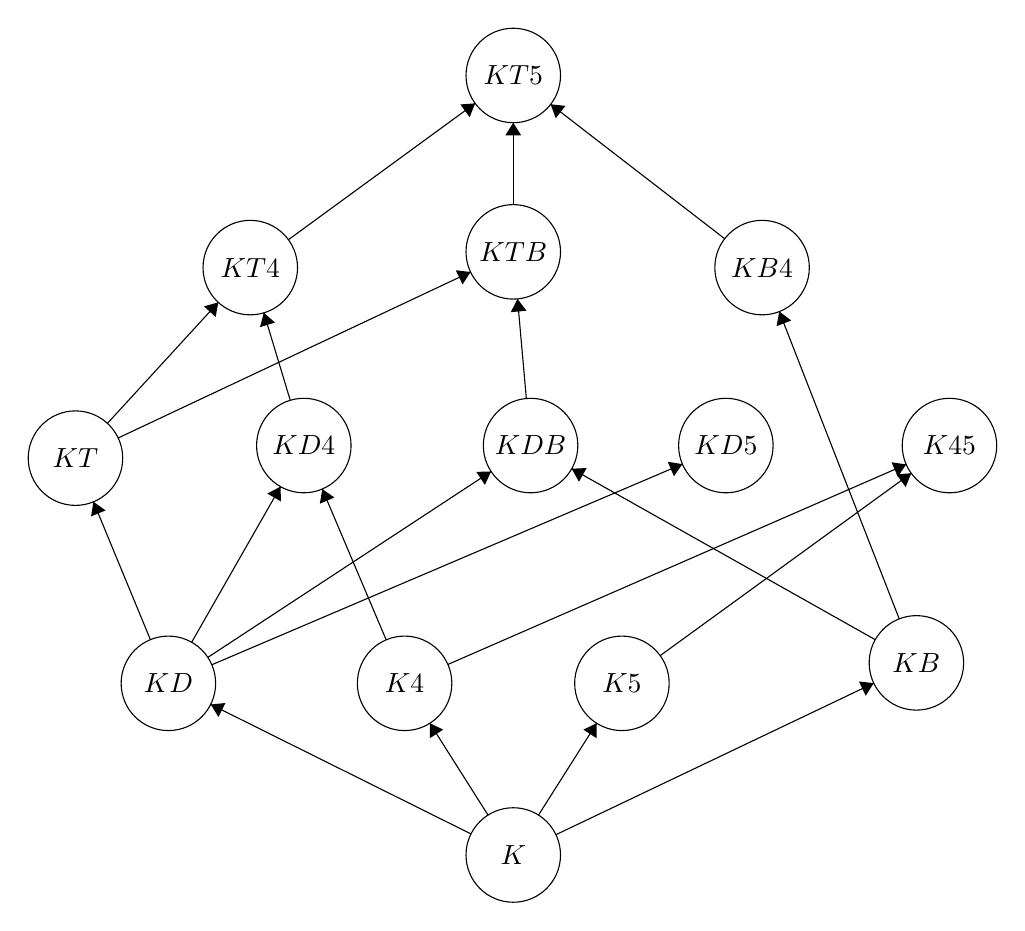
\begin{tikzpicture}[scale=0.2] \tikzstyle{every node}+=[inner sep=0pt] \draw [black] (39.9,-53.7) circle (3); \draw (39.9,-53.7) node {$K$}; \draw [black] (18,-42.8) circle (3); \draw (18,-42.8) node {$KD$}; \draw [black] (33,-42.8) circle (3); \draw (33,-42.8) node {$K4$}; \draw [black] (65.5,-41.5) circle (3); \draw (65.5,-41.5) node {$KB$}; \draw [black] (46.8,-42.8) circle (3); \draw (46.8,-42.8) node {$K5$}; \draw [black] (12.1,-28.5) circle (3); \draw (12.1,-28.5) node {$KT$}; \draw [black] (26.6,-27.7) circle (3); \draw (26.6,-27.7) node {$KD4$}; \draw [black] (53.4,-27.7) circle (3); \draw (53.4,-27.7) node {$KD5$}; \draw [black] (67.6,-27.7) circle (3); \draw (67.6,-27.7) node {$K45$}; \draw [black] (23.2,-16.4) circle (3); \draw (23.2,-16.4) node {$KT4$}; \draw [black] (39.9,-15.4) circle (3); \draw (39.9,-15.4) node {$KTB$}; \draw [black] (55.7,-16.4) circle (3); \draw (55.7,-16.4) node {$KB4$}; \draw [black] (39.9,-4.2) circle (3); \draw (39.9,-4.2) node {$KT5$}; \draw [black] (41,-27.7) circle (3); \draw (41,-27.7) node {$KDB$}; \draw [black] (37.21,-52.36) -- (20.69,-44.14); \fill [black] (20.69,-44.14) -- (21.18,-44.94) -- (21.62,-44.05); \draw [black] (38.3,-51.17) -- (34.6,-45.33); \fill [black] (34.6,-45.33) -- (34.61,-46.28) -- (35.45,-45.74); \draw [black] (42.61,-52.41) -- (62.79,-42.79); \fill [black] (62.79,-42.79) -- (61.85,-42.68) -- (62.28,-43.59); \draw [black] (41.5,-51.17) -- (45.2,-45.33); \fill [black] (45.2,-45.33) -- (44.35,-45.74) -- (45.19,-46.28); \draw [black] (16.86,-40.03) -- (13.24,-31.27); \fill [black] (13.24,-31.27) -- (13.09,-32.2) -- (14.01,-31.82); \draw [black] (14.13,-26.29) -- (21.17,-18.61); \fill [black] (21.17,-18.61) -- (20.26,-18.86) -- (21,-19.54); \draw [black] (25.74,-24.83) -- (24.06,-19.27); \fill [black] (24.06,-19.27) -- (23.82,-20.18) -- (24.77,-19.89); \draw [black] (31.83,-40.04) -- (27.77,-30.46); \fill [black] (27.77,-30.46) -- (27.62,-31.39) -- (28.54,-31); \draw [black] (19.48,-40.19) -- (25.12,-30.31); \fill [black] (25.12,-30.31) -- (24.28,-30.75) -- (25.15,-31.25); \draw [black] (20.76,-41.62) -- (50.64,-28.88); \fill [black] (50.64,-28.88) -- (49.71,-28.73) -- (50.1,-29.65); \draw [black] (35.75,-41.6) -- (64.85,-28.9); \fill [black] (64.85,-28.9) -- (63.92,-28.76) -- (64.32,-29.68); \draw [black] (49.23,-41.04) -- (65.17,-29.46); \fill [black] (65.17,-29.46) -- (64.23,-29.53) -- (64.82,-30.34); \draw [black] (64.41,-38.71) -- (56.79,-19.19); \fill [black] (56.79,-19.19) -- (56.62,-20.12) -- (57.55,-19.76); \draw [black] (62.89,-40.03) -- (43.61,-29.17); \fill [black] (43.61,-29.17) -- (44.07,-30) -- (44.56,-29.13); \draw [black] (20.51,-41.15) -- (38.49,-29.35); \fill [black] (38.49,-29.35) -- (37.55,-29.37) -- (38.1,-30.2); \draw [black] (14.81,-27.22) -- (37.19,-16.68); \fill [black] (37.19,-16.68) -- (36.25,-16.57) -- (36.68,-17.47); \draw [black] (40.73,-24.71) -- (40.17,-18.39); \fill [black] (40.17,-18.39) -- (39.74,-19.23) -- (40.74,-19.14); \draw [black] (25.62,-14.63) -- (37.48,-5.97); \fill [black] (37.48,-5.97) -- (36.54,-6.04) -- (37.13,-6.85); \draw [black] (39.9,-12.4) -- (39.9,-7.2); \fill [black] (39.9,-7.2) -- (39.4,-8) -- (40.4,-8); \draw [black] (53.33,-14.57) -- (42.27,-6.03); \fill [black] (42.27,-6.03) -- (42.6,-6.92) -- (43.21,-6.13); \end{tikzpicture} \end{center}

\textbf{\large{Somma diretta di Frame}}\textbf{}\\


S5 è determinata dalla classe dei frame d’ equivalenza (cioè frame
in cui la relazione di accessibilità è una relazione di equivalenza),
S5 = KT5 = KTB4 (riflessiva, simmetrica, transitiva)

S5 è determinata dalla classe dei frame universali (cioè frame in
cui la relazione di accessibilità è la relazione universale).

Mostriamo (almeno argomentiamo) la seconda affermazione.\\


Data una collezione di frame con insiemi di mondi a due a due disgiunti,
si dice somma diretta di questi frame il frame che ha come insieme
dei mondi l’unione dell’insieme dei mondi dei frame della collezione
e come relazione la unione delle relazioni dei frame della collezione.

$F=(S,R)$

$F1=(S1,R1)$, $F2=(S2,R2)$

$F=F1\oplus F2$ se e solo se $F=(S1\cup S2,\ R1\cup R2)$

Si dimostra che $\vera Fa$ se e solo se $\vera{F1}a$ e $\vera{F2}a$

Dato che una relazione di equivalenza forma una partizione sull'insieme
su cui è definita, e che in ogni classe di equivalenza è una relazione
universale, possiamo vedere una relazione di equivalenza come somma
di relazioni universali e il suo insieme come somma disgiunta di insiemi;
la somma diretta pertanto ci mostra quindi che S5 è determinata dai
frame universali.


\subsection{Tableau rivisitato per KT, KB}

Se una logica contiene l'assioma B devo aggiungere alle regole del
Tableau
\begin{itemize}
\item Regole di necessitazione\\
$\dfrac{\sigma\,\boa}{\sigma_{n}\, a}$ $\dfrac{\sigma\,\neg\dia}{\sigma_{n}\,\neg a}$
-- con $\sigma_{n}$ già presente nei nodi precedenti, oppure $\sigma_{n}$
\textbf{nodo corrente}
\end{itemize}
es. Si provi che la formula: $(\boa\implies a)$ è un teorema in KB

1: $\neg(\boa\implies a)$

1: $\boa$

1: $\neg a$

\textbf{1}: $a$ 

\begin{center}
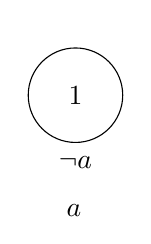
\begin{tikzpicture}[scale=0.2] 
\tikzstyle{every node}+=[inner sep=0pt] 
\draw [black] (26.8,-10.8) circle (3);
\draw (26.8,-10.8) node {1}; 

 
\draw (26.8,-6.6) node {$\boa$}; 

\draw (26.8,-15.1) node {$\neg{a}$};

\draw (26.7,-18.1) node {$a$}; 


\end{tikzpicture}
\end{center} 

Dove nell'ultimo passaggio ho usato proprio la regola appena introdotta,
avendo ottenuto $a$ e $\neg a$ nello stesso stato (mondo) deduco
che negare $a$ mi porta a un assurdo e quindi deve per forza essere
un teorema.\\
Se una logica contiene l'assioma T devo aggiungere alle regole del
Tableau
\begin{itemize}
\item Regole di necessitazione

\begin{itemize}
\item $\dfrac{\sigma\,\boa}{\sigma_{n}\, a}$ $\dfrac{\sigma\,\neg\dia}{\sigma_{n}\,\neg a}$
-- con $\sigma_{n}$ già presente nei nodi precedenti, oppure $\sigma_{n}$
\textbf{nodo prefisso del nodo corrente} (es 11 è prefisso di 111)
\end{itemize}
\end{itemize}
es. Si provi che la formula $(a\implies\boxx{\diamond a})$ è un teorema
in KT

1:$\neg(a\implies\boxx{\diamond a})$

1:$a$

1:$\neg(\boxx{\dia})$

1: $\diamond\boxx{\neg a}$

11: $\boxx{\neg a}$

\textbf{1: $\neg a$}

\begin{center} 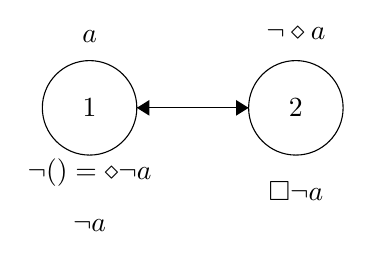
\begin{tikzpicture}[scale=0.2] \tikzstyle{every node}+=[inner sep=0pt] \draw [black] (26.7,-10.8) circle (3); \draw (26.7,-10.8) node {$1$};
\draw (26.7,-14.9) node {$\neg(\boxx{\dia})=\diamond\boxx{\neg a}$};
\draw (26.7,-18.3) node {$\neg a$}; \draw [black] (39.8,-10.8) circle (3); \draw (39.8,-10.8) node {$2$};
\draw (26.7,-6.3) node {$a$};
\draw (39.8,-6.1) node {$\neg\diamond a$};
\draw (39.8,-16.1) node {$\square\neg a$}; \draw [black] (29.7,-10.8) -- (36.8,-10.8); \fill [black] (36.8,-10.8) -- (36,-10.3) -- (36,-11.3); \draw [black] (36.8,-10.8) -- (29.7,-10.8); \fill [black] (29.7,-10.8) -- (30.5,-11.3) -- (30.5,-10.3); \end{tikzpicture} \end{center}


\end{document}
